% -*- TeX:UTF-8 -*-
%%
%% KAIST 학위논문양식 LaTeX용 (ver 0.4) 예시
%%
%% @version 0.4
%% @author  채승병 Chae,Seungbyung (mailto:chess@kaist.ac.kr)
%% @date    2004. 11. 12.
%%
%% @requirement
%% teTeX, fpTeX, teTeX 등의 LaTeX2e 배포판
%% + 은광희 님의 HLaTeX 0.991 이상 버젼 또는 홍석호 님의 HPACK 1.0
%% : 설치에 대한 자세한 정보는 http://www.ktug.or.kr을 참조바랍니다.
%%
%% @note
%% 기존에 널리 쓰여오던 차재춘 님의 학위논문양식 클래스 파일의 형식을
%% 따르지 않고 전면적으로 다시 작성하였습니다. 논문 정보 입력부분에서
%% 과거 양식과 다른 부분이 많으니 아래 예시에 맞춰 바꿔주십시오.
%%
%%
%% @acknowledgement
%% 본 예시 논문은 물리학과 박사과정 김용현 님의 호의로 제공되었습니다.
%%
%% -------------------------------------------------------------------
%% @information
%% 이 예제 파일은 hangul-ucs를 사용합니다. UTF-8 입력 인코딩으로
%% 작성되었습니다. hlatex의 hfont는 이용하지 않습니다. --2006/02/11
%% 본 템플릿은 전산학부 김민혁 교수에의해서 버그 수정되었습니다. -- 2016/11/25

% @class kaist.cls
% @options [default: doctor, korean, final]
% - doctor: 박사과정 | master : 석사과정
% - korean: 한글논문 | english: 영문논문
% - final : 최종판   | draft  : 시험판
% - pdfdoc : 선택하지 않으면 북마크와 colorlink를 만들지 않습니다.


\documentclass[master,korean,final,pdfdoc]{kaist-ucs}
%\documentclass[master,korean,final]{kaist-ucs}
% \documentclass[master,korean,draft]{kaist-ucs}


% If you want make pdf document (include bookmark, colorlink)
%\documentclass[doctor,english,final,pdfdoc]{kaist-ucs}

% kaist.cls 에서는 기본으로 dhucs, ifpdf, graphicx 패키지가 로드됩니다.
% 추가로 필요한 패키지가 있다면 주석을 풀고 적어넣으십시오,


% @command title 논문 제목(title of thesis)
% @options [default: (none)]
% - korean: 한글제목(korean title) | english: 영문제목(english title)
\title[korean] {떨어져 사는 가족에게 은근한 함께 삶을 제공하는 로봇 아바타 시스템 디자인}
\title[english]{Design of a Robotic Avatar System Providing Subtle Living-togetherness for Families Living Apart}

% @note 표지에 출력되는 제목을 강제로 줄바꿈하려면 \linebreak 을 삽입.
%       \\ 나 \newline 등을 사용하면 안됩니다. (아래는 예시)
%
%\title[korean]{탄소 나노튜브의 물리적 특성에 대한\linebreak 이론 연구}
%\title[english]{Theoretical study on physical properties of\linebreak
%                carbon nanotubes}
%
% If you want to begin a new line in cover, use \linebreak .
% See examples above.
%


% @command author 저자 이름
% @param   family_name, given_name 성, 이름을 구분해서 입력
% @options [default: (none)]
% - korean: 한글이름 | chinese: 한문이름 | english: 영문이름
% 한문 이름이 없다면 빈 칸으로 두셔도 됩니다.
%
%
% If you are a foreigner , write your name in korean or your korean name.
% If you can't write native character, you can make the chinese blank empty 
% Write as follow
% \author[korean]{family name in korean}{given name in korean}
% \author[chinese]{family name in your native language}{given name in your native language}
% \author[english]{family name in english}{given name in english}
%
\author[korean] {장}{영 재}
\author[korean2] {장}{영재}    %이름을 붙여 써 주시기 바랍니다.
\author[chinese]{張}{榮宰}
\author[english]{Chang}{Youngjae}

% @command advisor 지도교수 이름 (복수가능)
% @usage   \advisor[options]{...한글이름...}{...영문이름...}{signed|nosign}
% @options [default: major]
% - major: 주 지도교수  | coopr: 공동 지도교수
\advisor[major]{송 준 화}{Junehwa Song}{signed}
\advisor[major2]{송준화}{Junehwa Song}{signed} %한글 성과 한글 이름을 모두 붙여 써 주시기 바랍니다.
\advisorinfo{Professor of School of Computing} %제출승인서에 들어가는 교수님 정보, advisor's information   
%\advisor[coopr]{홍 길 동}{Gil-Dong Hong}{nosign}
%\advisor[coopr2]{홍길동}{Gil-Dong Hong}{nosign}    %한글 성과 한글 이름을 모두 붙여 써 주시기 바랍니다.
%
% 지도교수 한글이름은 입력하지 않아도 됩니다.
% You may not input advisor's korean name
% like this \advisor[major]{}{Chang, Kee Joo}{signed}
%


% @command department {학과이름}{학위종류} - 아래 규칙에 따라 코드를 입력
% @command department {department code}{degree field}
%
% department code
% 2. 석박사학위논문 작성 및 제출요령 4쪽 ~ 5쪽 참고
% 또는 kaist-ucs.cls 의 % @command department 참고

% science: 이학 | engineering: 공학 | business : 경영학
% 박사논문의 경우는 학위종류를 입력하지 않아도 됩니다.
% If you write Ph.D. dissertation, you cannot input degree field.
% The third parameter : a | b | c
% a: 소속된 학과만 쓰는 옵션 (학과에만 소속되어 있는 경우에는 무조건 a를 선택해야 함)
% b: 학과 아래의, 프로그램이나 학제전공에 소속되어 있을 경우에 학과와 프로그램을 함께 쓰는 옵션
% c: 학과 아래의, 프로그램이나 학제전공에 소속되어 있을 경우에 학과를 쓰지 않고 프로그램이나 학제전공의 이름만 쓰는 옵션 
% 
% a: it represents only the name of department. (if you aren't in the program under the department, must choose a)
% b: it represents the names of department and the program that is under the department (consider this when you are in the program not only department)
% c: it represents only the name of program that is under the department (consider this when you are in the program not only department)ㄷ

\department{CS}{engineering}{a}

% @command studentid 학번(ID)
\studentid{20173498}

% @command referee 심사위원 (석사과정 3인, 박사과정 5인)
\referee[1]{송 준 화}
\referee[2]{조 성 호}
\referee[3]{이 영 기}
% \referee[5] {Barack Obama}
% Of course english name is available

% @command approvaldate 지도교수논문승인일
% @param   year,month,day 연,월,일 순으로 입력
\approvaldate{2018}{6}{30} 
\fontsize{18pt}{18pt}\selectfont

% @command refereedate 심사위원논문심사일
% @param   year,month,day 연,월,일 순으로 입력
\refereedate{2018}{6}{5}

% @command gradyear 졸업년도
\gradyear{2018}

% --------
% Packages
% --------
\usepackage{kotex} % For automatic josa matching
\usepackage{caption} % For right amount of space after a caption
\usepackage{booktabs} % For formal tables
\usepackage{tabu} % For equal-sized tabular
\usepackage{enumitem} % For spacing options between list items
\usepackage{multirow} % For multi-row spanning cell
\usepackage{subcaption} % For subfigures in figures

% ---------------
% Custom Commands
% ---------------

% comments
\definecolor{olivegreen}{rgb}{0, 0.6, 0}
\definecolor{orange}{rgb}{1, 0.5, 0}
\definecolor{skyblue}{rgb}{0, 0.75, 1}
\definecolor{salmon}{rgb}{1, 0.6, 0.6}
\definecolor{red}{rgb}{1, 0, 0}
\definecolor{blue}{rgb}{0, 0, 1}
\definecolor{black}{rgb}{0, 0, 0}
\newcommand{\tglee}[1]{{\color{olivegreen}[\textbf{\sc taegyeong}: \textit{#1}]}}
\newcommand{\shkim}[1]{{\color{orange}[\textbf{\sc seonghoon}: \textit{#1}]}}
\newcommand{\sclee}[1]{{\color{salmon}[\textbf{\sc seungchul}: \textit{#1}]}}
\newcommand{\yjc}[1]{{\color{skyblue}[\textbf{\sc youngjae}: \textit{#1}]}}
\newcommand{\wonjung}[1]{{\color{red}[\textbf{\sc wj}: \textit{#1}]}}
\newcommand{\highlight}[1]{{\color{red}{#1}}}

% remove comments
% \renewcommand{\tglee}[1]{{}}
% \renewcommand{\shkim}[1]{{}}
% \renewcommand{\sclee}[1]{{}}
% \renewcommand{\yjc}[1]{{}}
% \renewcommand{\wonjung}[1]{{}}
% \renewcommand{\highlight}[1]{{#1}}

% placeholders
\newcommand{\concept}{은근한 함께 삶}
\newcommand{\sysname}{HomeMeld\jung}
\newcommand{\location}{의미적으로 유사한 위치}
\newcommand{\approach}{로봇 아바타 기반 항시적 위치 동기화 방식}
\newcommand{\expWorkshop}{디자인 워크샵}
\newcommand{\expMapping}{매핑 실험}
\newcommand{\expUser}{시나리오 중심 사용자 스터디}

% 본문 시작
\begin{document}

% 앞표지, 속표지, 학위논문 제출승인서, 학위논문 심사완료 검인서는
% 클래스 옵션을 final로 지정해주면 자동으로 생성되며,
% 반대로 옵션을 draft로 지정해주면 생성되지 않습니다.
% 학위논문 제출 승인서에서 자신의 전공과 교수님의 정보를 바꾸기 위해서는 첨부되어있는 제목이 kaist-ucs인 class 문서에 들어가서 ####################로 표시  
% 한 부분을 바꾸시길 바랍니다.

%% 초록
\thesisinfo
% 논문 서지, 초록, 핵심 낱말, 영문 초록, 영어 핵심 낱말 (Information of thesis, abstract in korean, keywords in korean, abstract in english, keywords in english)
% 한글 초록은 500자를, 영문 초록은 300 낱말을 넘지 않아야 함
% 핵심 낱말은 5 개 이내로 넣음
% 한글 초록에 영문 글자를 쓰지 않도록 한다.

\begin{summary}      
학업, 직장으로 어쩔 수 없이 떨어져 사는 가족들은 영상통화, SNS, 메신저 등의 첨단 연결기술에 삶의 많은 부분을 기댄다. 하지만 이들 기술의 높은 완성도와 가용성에도, 현재 이들의 삶은 함께 살아가는 삶과 비교하면 아직 많이 부족하다. 본 연구는 함께 삶이 제공하는 다양한 감각 중 일상 속에서 지속적으로 상대방의 존재를 느낄 수 있을 때 형성되는 \emph{은근한 함께 삶}이라는 감각에 주목한다. 또한 이를 원거리에서 실현하기 위한 방법으로 \emph{로봇 아바타 기반 항시적 위치 동기화}를 제시한다. 이어 동기화를 위한 핵심 기술로서 \emph{가구를 중심으로 한 의미적 위치 및 방향 재현 기술}을 고안했다. 이어 제안하는 방식이 은근한 함께함에 미치는 효과를 확인하기 위해 5쌍의 실제 부부를 대상으로 시나리오 중심 사용자 스터디을 진행했다. 실험 참가자들은 상대방의 위치에서 들려오는 목소리, 대화의 공백에 대한 적은 부담, 로봇의 움직임에 따른 대화 기회 제공 등의 시스템 요소에 긍정적으로 반응했다. 본 논문은 \emph{은근한 함께 삶}을 위한 새로운 장르의 원거리 인터랙션 기술 및 서비스의 초기 연구로서 향후 관련 연구에 기초 자료로 활용될 수 있다.
\end{summary}

\begin{Korkeyword}
은근한 함께 삶, 로봇 아바타, 떨어져 사는 가족, 소셜 컴퓨팅
\end{Korkeyword}

%%%%%%%%%%%%%%%%%%%%%%%%%%%%%%%%%%%%%%%%%%%%%%

\begin{abstract}
Families living apart relies heavily on cutting-edge communication tools such as video calls, social network services, and messengers. However, despite the high availability and accessibility of such services, separated families still suffer from subtle voids which make the experience incomparable to the those of living together. Here I focus on exploring \emph{subtle living-togetherness}, a sense of togetherness formed when we can feel the other's presence consistently in everyday lives. We propose a \emph{robot avatar based continuous location synchronization} to support the subtle living-togetherness experience. To realize the synchronization, we designed a functional-object based semantic location mapping algorithm. We conducted a scenario-based user study with 5 couples in a lab environment and observed that our design considerations positively affected to the subtle living-togetherness. The paper concludes by discussing the implications for opening up this new genre of remote communication systems.
\end{abstract}
 
\begin{Engkeyword}
Subtle living-togetherness, Robotic avatar, Families living apart, Social Computing
\end{Engkeyword}


%% 형식
\addtocounter{pagemarker}{1}    % 페이지 숫자 세팅
\newpage                        % 백색별지분을 고려

%% 목차
\tableofcontents                % 목차 (Table of Contents) 생성
\listoftables                   % 표목차 (List of Tables) 생성
\listoffigures                  % 그림목차 (List of Figures) 생성
% 위의 세 종류의 목차는 한꺼번에 다음 명령으로 생성할 수도 있습니다.
%\makecontents

%% NOTICE
% 한글로 쓴 논문에는 본문에 영문 글자를 쓰지 않는다.
% 다만, 꼭 필요할 때에는 ‘한글 낱말 (영문 낱말)’ 꼴로 적는다.
% 이하의 본문은 LaTeX 표준 클래스 report 양식에 준하여 작성하시면 됩니다.
% 하지만 part는 사용하지 못하도록 제거하였으므로, chapter가 문서 내의
% 최상위 분류 단위가 됩니다.

%% 인용
%인용은 다음과 같이 합니다 \cite{RVP1}-\cite{ML2}.
%인용은 뒤에 인용을 쓰는 칸이 있습니다. 참고하여서 인용하시길 바랍니다 \cite{SOCA2,EF2}.
%한글 논문에는 영어를 쓰지 마시기 바랍니다. 

%% 본문
\chapter{서론}
\label{sec:introduction}

% A:아내, B:남편
\newcommand{\A}{지효}
\newcommand{\B}{승표}


% 교수님 커멘트 Problem & Solution approach가 명확하지 않은 글. 
% 이것을 좀 더 강화해야
% problem이 뭔지? solution approach가 뭔지?

%%%% 1번째 단락: 은근한 함께함 체험시키기 시나리오 %%%%
%%%% --------------------------------------------------

% 시나리오 버전 1
% 도시에서 바쁜 일상을 살아가는 부부인 \A와 \B를 생각해보자. 그들은 각자의 직장에서 바쁜 한 주를 보낸 후, 마침내 주말을 맞이하였다. \B는 모처럼 아내와 즐거운 시간을 보내기 위해 야심차게 데이트를 준비했지만, 여전히 일이 남은 \A는 주말에도 집에서 업무를 해야 했다. 어쩔 수 없이 \B는 바쁜 아내를 위해 커피를 같이 마시고 옆에서 책을 읽으며 토요일 오후를 보내게 되었다. \B는 비록 아내와 계획했던 데이트를 하지는 못했지만, 아내와 주말 오후를 같이 보내며 잔잔한 만족감을 느꼈다. \A는 바쁘게 일을 하면서도, 자신의 옆에 같이 있어준 남편 덕분에 편안함과 안정감을 느꼈다. 이들은 서로에게 집중하지도, 같은 활동을 하지도, 긴 대화를 나눈 것도 아니었지만, 편안하고 잔잔하게 느껴지는 `\concept'을 즐기며 더 깊은 유대감을 만들고 행복한 기억을 만들었다. \highlight{이후 두 사람은 \A가 바쁜 주말을 보내야 할 때마다 자주 이러한 시간을 보내곤 했다.} 그런데 어느 날, \A는 직장에서 미국 지사로 발령받았고 \A와 \B는 결국 떨어져 살게 되었다. 같이 살 때의 마음을 이어가기 위해 그들은 서로 자주 통화하고 꾸준히 대화를 했지만, 그들은 자주 집에 같이 보냈던 토요일 오후가 그리웠다. 이 부부는 더 이상 `\concept'을 느낄 수 없게 된 것일까?

% 시나리오 버전 2
%맞벌이 부부 \A와 \B는 각자 업무에 치여 정신없는 한 주를 보낸 뒤 토요일을 맞이하였다. 그들은 모처럼 달콤한 데이트를 하기 위해 놀이공원에 갈 계획 이었으나, 이는 일장춘몽에 불과했다. 토요일 아침 \A의 상사로부터 걸려 온 전화, 이로 인해 \A는 꼼짝없이 집에서 일을 해야만 했다. 어쩔 수 없이 \B는 바쁜 아내를 위해 커피를 같이 마시고 옆에서 책을 읽으며 토요일 오후를 보냈다. \B는 비록 아내와 계획했던 달콤한 데이트를 하지는 못했지만, 아내와 주말 오후를 같이 보내며 잔잔한 만족감을 느꼈다. \A는 바쁘게 일을 하면서도, 자신의 옆에 같이 있어준 남편 덕분에 편안함과 안정감을 느꼈다. 이들은 서로에게 집중하며 활동적인 데이트를 즐긴 것도, 긴 대화를 나눈 것도 아니었지만, 편안하고 잔잔하게 느껴지는 `\concept'을 즐기며 더 깊은 유대감을 만들고 좋은 기억을 만들었다. \highlight{이후 두 사람은 \A가 바쁜 주말을 보내야 할 때마다 자주 이러한 시간을 보내곤 했다.} 그런데 어느 날, \A는 직장에서 미국 지사로 발령받았고 \A와 \B는 결국 떨어져 살게 되었다. 같이 살 때의 마음을 이어가기 위해 그들은 서로 자주 통화하고 꾸준히 대화를 했지만, 그들은 종종 집에서 같이 보냈던 토요일 오후가 그리웠다. 이 부부는 더 이상 `\concept'을 느낄 수 없게 된 것일까?

%시나리오 버전 3
맞벌이 부부이자 독서를 좋아하는 \B\와 \A에게 느긋하게 커피를 마시며 함께 책을 읽는 토요일 오후는 \concept\을 느끼는 매우 소중한 시간이다. 정신없이 바쁜 직장생활 때문에 혼자인가 싶다가도, 이 시간을 통해 서로 함께하고 있다는 것을 다시금 확인하게 된다. 사실 많은 대화가 오고 가는 시간은 아니다. 그들은 각자 자신의 책을 읽는데 집중한다. 그렇지만, 하고 싶은 일을 마음껏 하면서도 사랑하는 사람이 곁에 있다는 점과 언제든 자신의 생각을 공유할 상대가 있다는 점이 \A\와 \B에게는 큰 편안함과 안정감을 준다. 잔잔하게 느껴지는 \concept\은 그들의 관계를 더욱 돈독하게 만들어왔다. 그러던 어느 날, 이 부부에게 청천벽력 같은 소식이 떨어졌다. \A\가 직장에서 미국 지사로 발령받아 더 이상 이 토요일 오후 시간을 함께 할 수 없게 된 것이다. 함께 책을 읽던 시간을 떠올리며 통화를 하지만, 그들은 종종 집에서 같이 보냈던 토요일 오후가 그리웠다. 이 부부는 더 이상 `\concept'\을 느낄 수 없게 된 것일까?

%%%% 2번째 단락: 문제 제기 %%%%
%버전 1 --> 기존의 연구들과 비교를 좀 해줘야 하지 않을까?
\A\와 \B\ 부부처럼, 직장 혹은 학업 때문에 어쩔 수 없이 떨어져 살게 되는 가족은 전세계적으로 늘어나고 있다. 현재 미국에만 총 360만 명의 부부가 떨어져 살고 있으며, 영국의 경우에도 전체 부부의 10\%가 떨어져서 살고 있다 \cite{duncan2013people, strohm2009living}. 이는 한국도 크게 다르지 않은데, 비동거 맞벌이 가구 수는 전체 가구의 4.6\%에 달하며, 서울의 경우 10쌍 중 1쌍이 기러기 가족 생활을 하고 있다 \cite{rock2016goose, wise2012seoul}. 이들은 인터넷 및 IoT 기술의 발전으로 메신저, 영상통화, 소셜 미디어 등을 통해 서로 연락하기 쉬워졌지만, 여전히 \A\와 \B\ 부부가 함께 있을 때 느꼈던 \concept\을 느낄 수 없고 이로 인한 아쉬움과 그리움을 떨쳐 낼 수가 없다.
\tglee{충국이형: 왜 통화로 할 수 없었는지를 elaborate 하면 좋지 않을까}비록 물리적으로 떨어져 있지만, 그럼에도 같이 살았을 때의 \concept\을 만들어 줄 수는 없을까? 

%버전 2 --> 메신저, 영상통화, 소셜미디어 빼고 기존의 연구들 두 문장 추가함. 너무 추상적인 것 같기도...
%\A와 \B\ 부부처럼, 직장 혹은 학업 때문에 어쩔 수 없이 떨어져 살게되는 가족은 전세계적으로 늘어나고 있다. 현재 미국에만 총 360만명의 부부가 떨어져 살고 있으며, 영국의 경우에도 전체 부부의 10\%가 떨어져서 살고 있다 \cite{strohm2009living, duncan2013people}. 이는 한국도 크게 다르지 않은데, 비동거 맞벌이 가구 수는 전체 가구의 4.6\%에 달하며, 서울의 경우 10쌍 중 1쌍이 기러기 가족 생활을 하고 있다 \cite{rock2016goose, wise2012seoul}. 학계에서는 이러한 가족들에게 함께함(co-presence)을 경험하게 하는 것을 중요한 문제로 여기고 활발히 연구하고 있다. 하지만, 기존의 연구들은 대부분 특정 활동을 함께 할 때 경험하게 되는 함께함에 초점이 맞추어져 있다 \cite{kirk2010home, neustaedter2012intimacy, judge2010sharing, yang2017communicating}. 이는 \A와 \B부부가 상대방을 은근하게 느끼면서 경험하던 \concept과는 다른 종류의 함께 함이다. 


%%%% 3번째 단락: solution approach 1 %%%%

%%%%%%%%%%%%%%%%%%%%%%%%%%%%%%%%%%%%%%%%%%%%%%%%%%%%%%%%%%%%%%%%%%%%%%%%%
\begin{figure}
\begin{subfigure}{.5\textwidth}
  \centering
  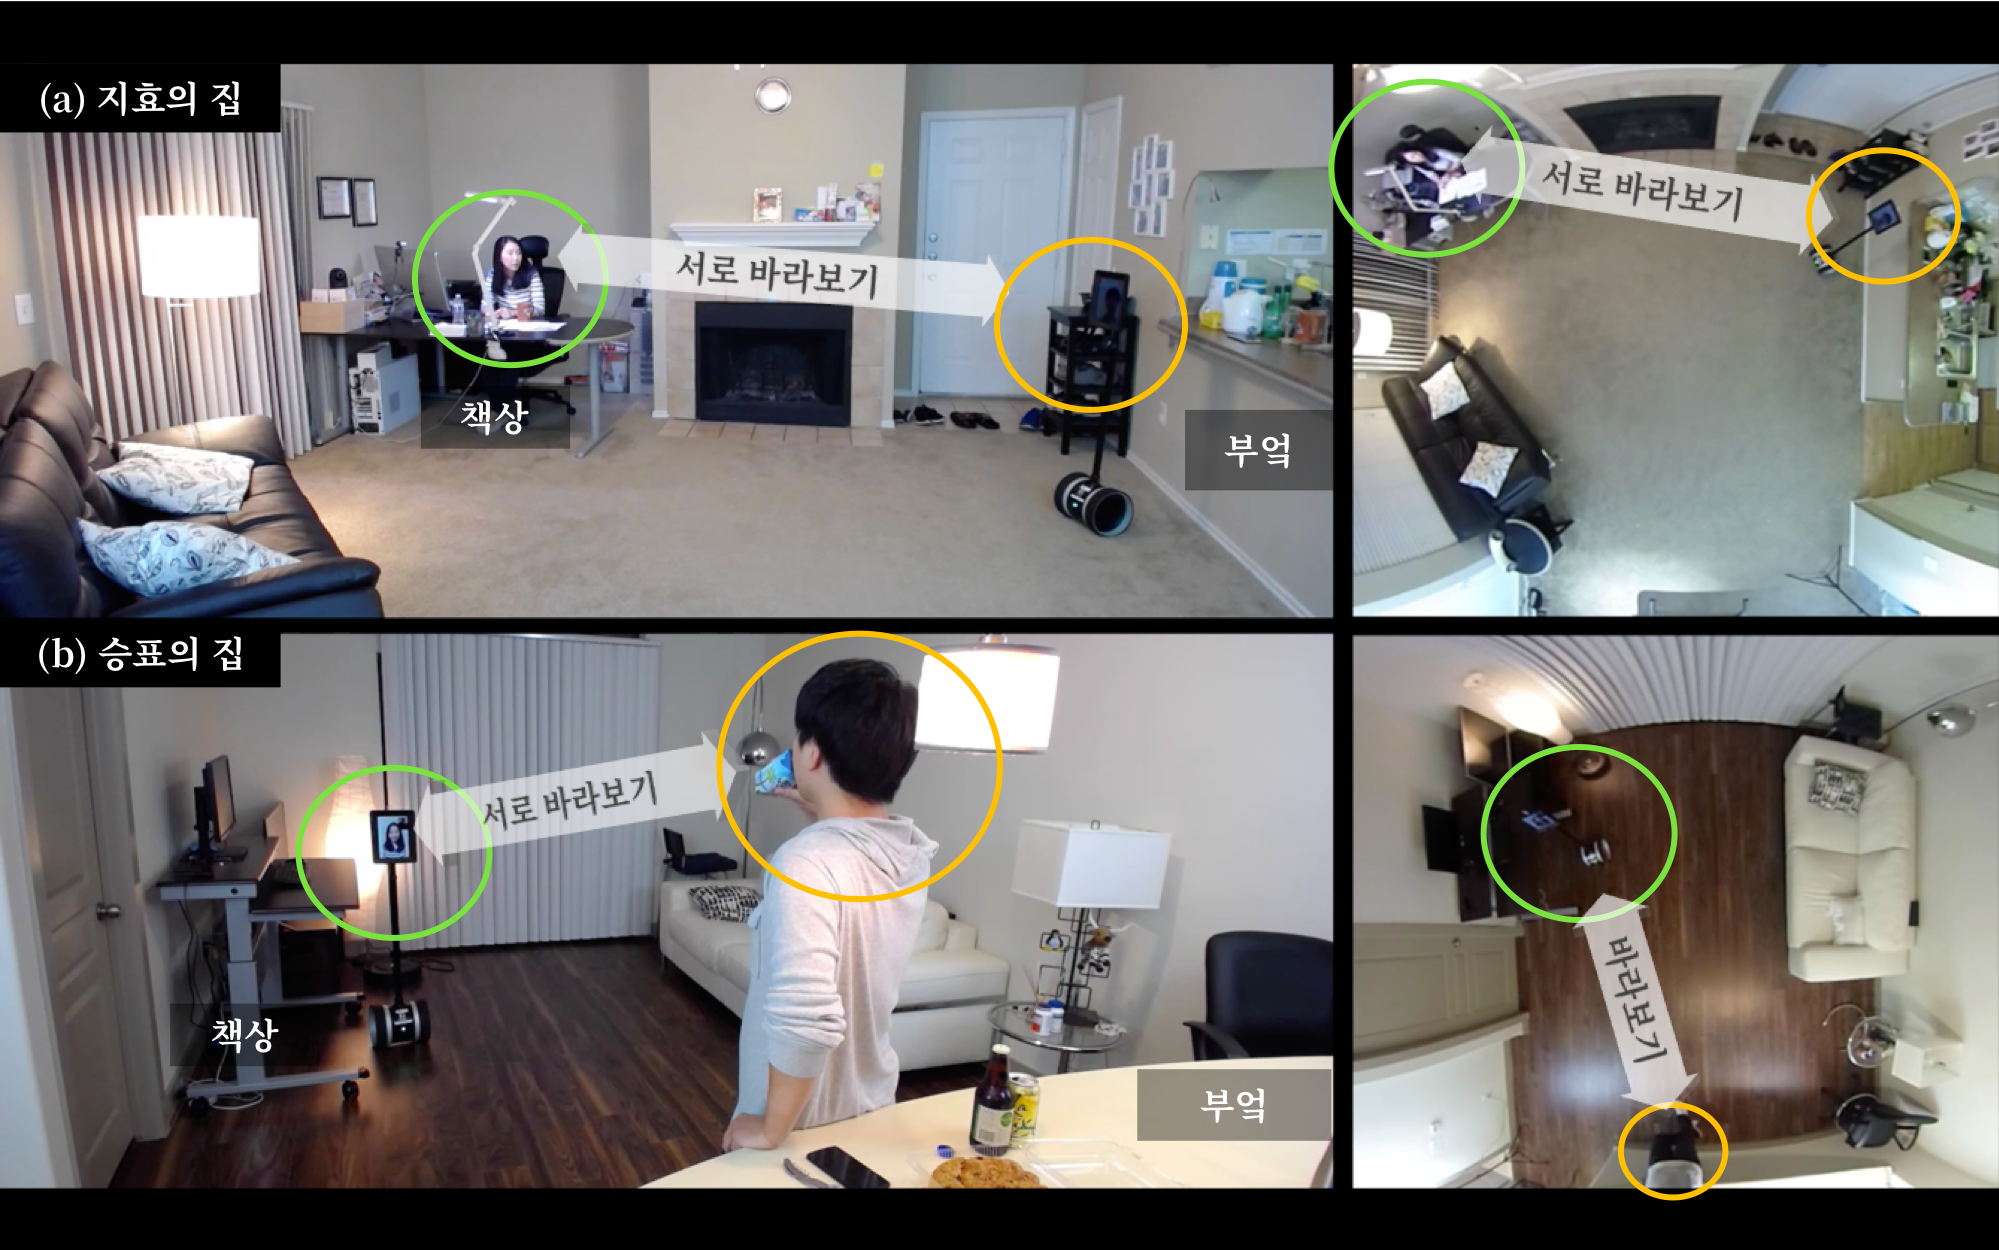
\includegraphics[width=\textwidth]{images/concept1}
\end{subfigure}
\begin{subfigure}{.5\textwidth}
  \centering
  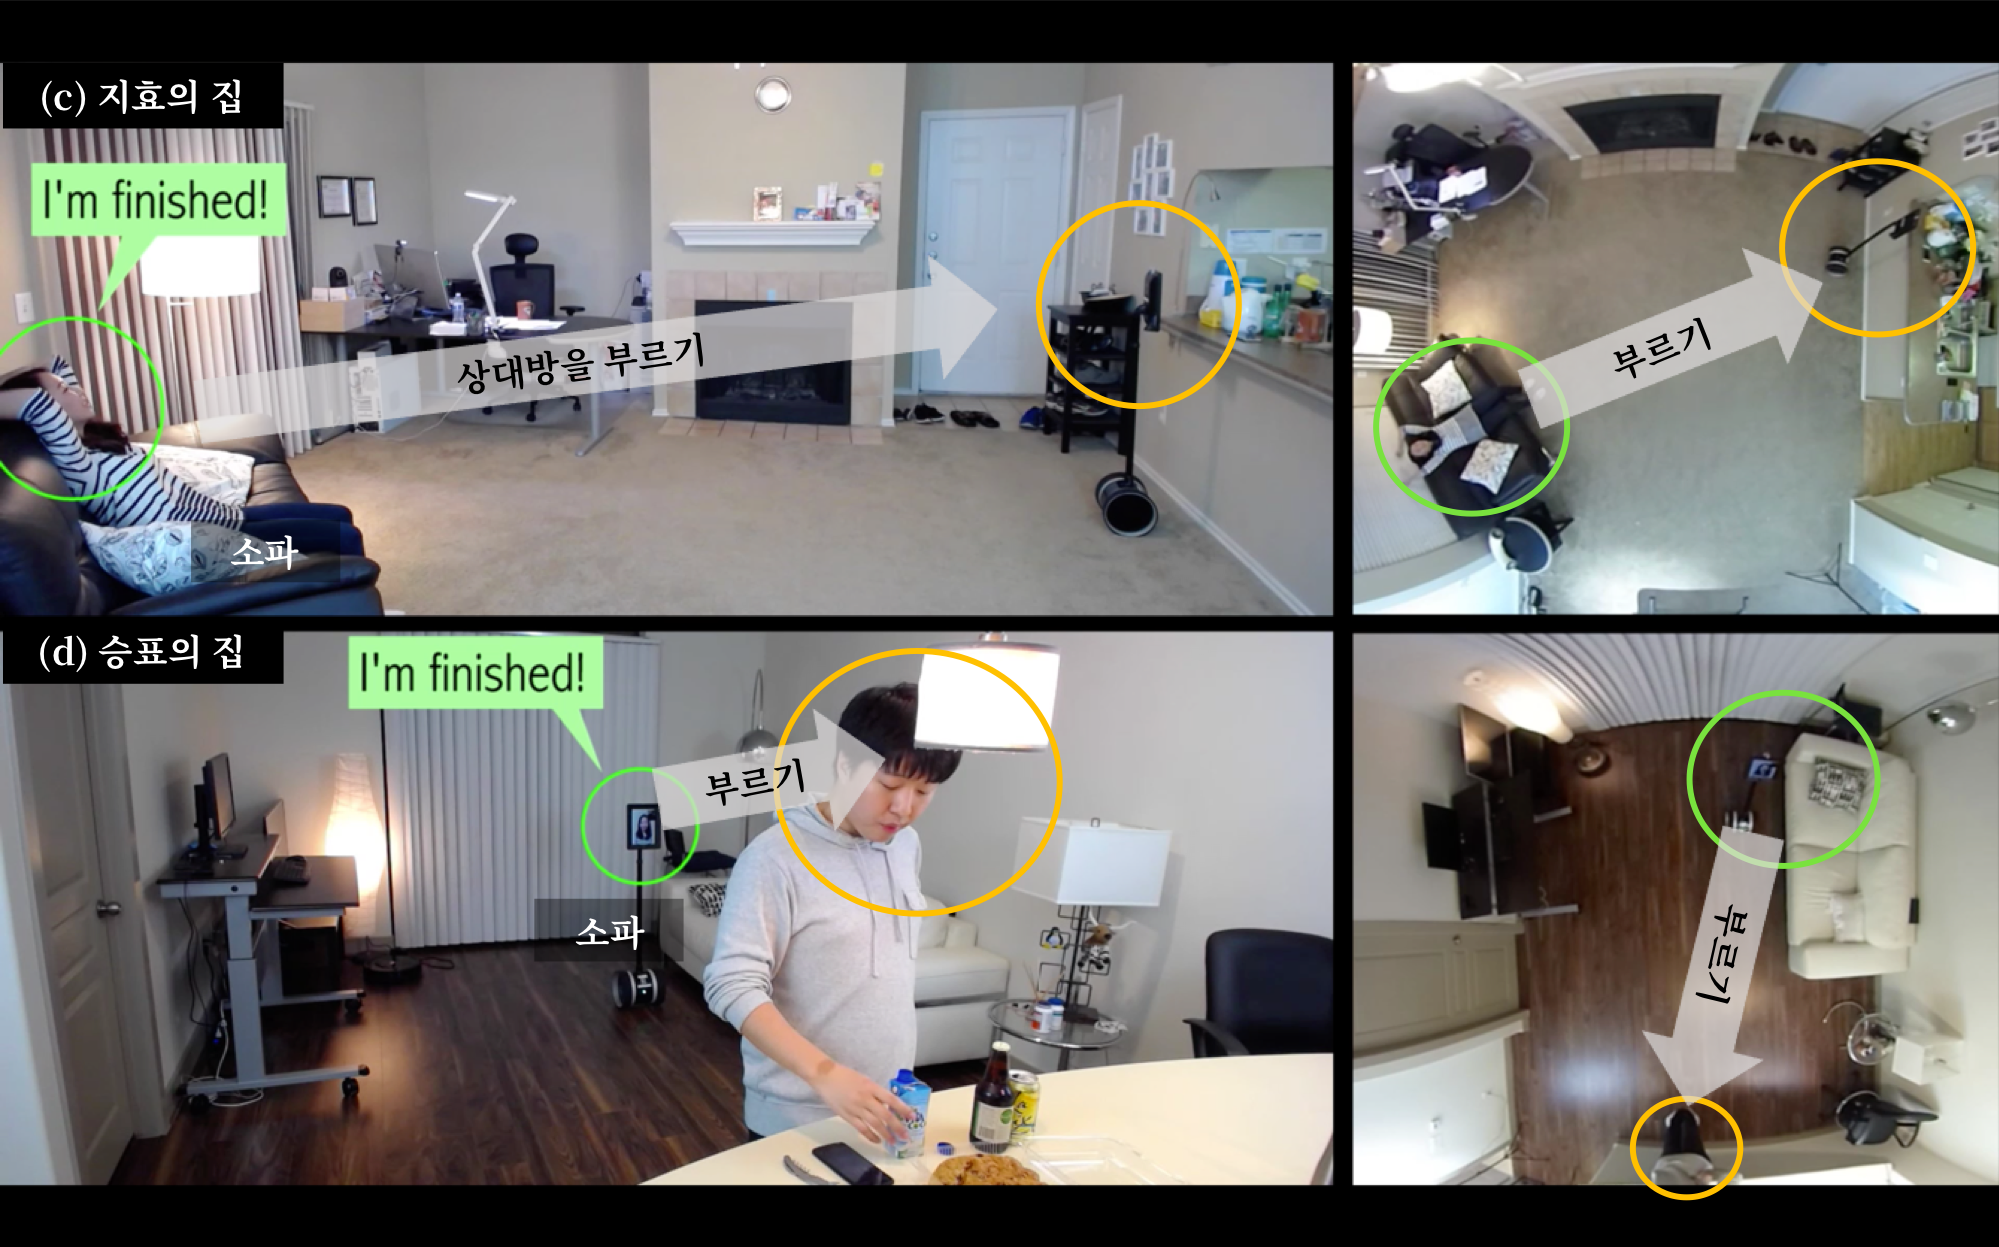
\includegraphics[width=\textwidth]{images/concept2}
\end{subfigure}
\caption{\approach을 이용한 시스템의 콘셉트}
\label{fig:concept}
\end{figure}
%%%%%%%%%%%%%%%%%%%%%%%%%%%%%%%%%%%%%%%%%%%%%%%%%%%%%%%%%%%%%%%%%%%%%%%%%

% 버전1
% 나는 서로 떨어져 사는 가족들에게 \concept을 제공하기 위한 하나의 방법으로 로봇 아바타 기반 항시적 위치 동기화 방식, \sysname를 제시한다. \sysname는 떨어져 사는 두 사람을 각자의 집에 투영하여 \concept을 제공하고자 각각 서로를 대변하는 아바타로써 텔레프레즌스(Telepresence) 로봇\cite{double_robotics}을 사용한다. 집 A에 있는 사람의 로봇 아바타가 집 B에 있고, 집 B에 사는 사람의 아바타가 집 A에 있으며, 이 로봇 아바타는 상대방의 집안 위치와 의미적으로 유사한 곳에 위치한다. 즉, 집 B 에 사는 상대방이 소파에서 TV 를 보다가 화장실로 움직이면, 집 A에서 소파에 있다가 화장실로 이동한다. 사용자들은 로봇 아바타를 통해 상대방의 집안 움직임과 위치를 직관적으로 파악하고 이를 통해 상대방의 행동과 상태를 쉽고 자연스럽게 알 수 있게 된다. 예를 들어, 로봇 아바타가 집안 냉장고 앞에 있다면, 상대방이 냉장고에서 음식이나 음료를 찾는 중이라는 것을 알 수 있다.

%버전2 --> 집 A, 집 B를 없애고 싶었음.
% 본 연구에서 나는 서로 떨어져 사는 가족들에게 \concept\을 제공하기 위한 하나의 방법으로 `\approach'\을 제시한다. 이는 텔레프레젠스 로봇(Telepresence Robot \cite{double_robotics})이 상대방의 아바타가 되어, 
% \highlight{내 집에서 상대방의 위치를 나타내는 방식이다.}
% 상대방이 소파에서 TV를 보다가 화장실에 가면, 내 집에 있는 상대방의 로봇 아바타도 소파에 있다가 화장실로 움직이게 된다. 사용자들은 로봇 아바타를 통해 상대방의 움직임과 위치를 직관적으로 파악하고, 이를 통해 상대방의 행동과 상태를 쉽고 자연스럽게 알 수 있다. 예를 들어, 로봇 아바타가 집안 냉장고 앞에 있다면, 상대방이 냉장고에서 음식이나 음료를 찾는 중이라는 것을 알 수 있다.

% 버전3 교수님과 연구실 사람들과 같이 고쳐봄
나는 이를 실현할 수 있는 한 가지 방법으로 `\approach'\을 제시한다. 이는 텔레프레즌스 로봇(Telepresence Robot \cite{double_robotics})을 상대방의 아바타로 삼고 내 집 적절한 장소에 놓아, 상대방의 행동과 상황을 잘 표현하는 방식이다. 떨어져 사는 상대방의 행동을 가장 비슷하게 나타낼 수 있는 내 공간상의 장소에 위치하는 아바타를 상상해보자. 예를 들어, 상대방이 집에서 먹을 음식을 찾고 있으면, 아바타는 냉장고 앞에 위치하게 된다. 사람들은 이러한 아바타를 통해 상대방의 행동을 쉽게 유추하고 \concept\을 느낄 수 있을 것이다.


%%%% 4번째 단락: solution approach 2 %%%%
%제안하는 방식이 어떻게 또는 왜 \concept을 제공할 수 있는지 한문단.

% 버전1
% \approach의 핵심 요소는 `텔레프레즌스 로봇의 활용'과 `의미적으로 유사한 위치 및 방향(semantically equivalent location/orientation)의 재현'이다.
% \tglee{충국이형: 두 요소가 독립적인가? 같은 level 이 아닌 것 같음}
% 이는 떨어져 산 경험이 있는 가족 구성원들을 대상으로 진행한 \expWorkshop\을 통해 도출되었다.
% 텔레프레즌스 로봇의 활용은 물리적인 실체를 통해 상대방의 존재와 인기척을 효과적으로 나타내며, 사용자에게 장비 착용을 요구하지 않기에 일상에서 이를 지속적으로 사용하는 것을 가능케 한다.
% 또한, 의미적으로 유사한 위치와 방향의 재현은 상대방의 행동과 상태를 쉽게 전달하고 이를 사용자들이 인지하는데 큰 노력과 집중을 들이지 않도록 만든다. \highlight{이처럼 상대방을 나타내는 로봇 아바타는 자연스럽게 사용자의 일상에 녹아들어 `\concept'\을 연출한다.}

% 버전2
\approach의 핵심 요소는 `의미적으로 유사한 위치 및 방향(semantically equivalent location/orientation)의 재현'이다.
이는 떨어져 산 경험이 있는 가족 구성원들을 대상으로 진행한 \expWorkshop\을 통해 도출되었다.
먼저, 나는 \concept을 제공하기 위한 합리적인 디자인 요소로써 텔레프레즌스 로봇을 선택하였다.
로봇의 사용은 물리적인 실체를 통해 상대방의 존재와 인기척을 효과적으로 나타내며, 사용자에게 장비 착용을 요구하지 않기에 일상에서 이를 지속적으로 사용하는 것을 가능케 한다.
이러한 로봇의 활용은 이를 어떤 장소에 위치시키는가에 대한 질문으로 연결된다. 이에 본 연구는 \expWorkshop을 통해 얻은 `의미적으로 유사한 위치와 방향의 재현'을 제안한다.
로봇을 통해 가구중심을 기반으로 의미적으로 유사한 위치와 방향을 재현하는 것은 상대방의 행동과 상태를 쉽게 전달하고 이를 사용자들이 인지하는데 큰 노력과 집중을 들이지 않도록 만든다. \highlight{이는 자연스럽게 사용자의 일상에 녹아들어 `\concept'\을 연출한다.}


% 이를 토대로 `\approach'를 고안하였으며 각 핵심요소는 다음과 같이 \concept을 제공한다.
% (1) 물리적인 실체가 있는 로봇의 활용은 상대방의 존재와 인기척을 효과적으로 나타내며,
% (2) 의미적으로 유사한 위치와 방향을 재현함으로써 상대방의 행동과 상태를 쉽게 전달한다. 또한, 
% (3) 로봇의 위치와 움직임을 통해 상대방의 맥락을 전달하기 때문에 이를 사용자들이 인지하는데 큰 노력과 집중이 요구되지 않으며 일상에 은근하게 녹아들 수 있다. 마지막으로 이 방식은 사용자에게 장비착용을 요구하지 않기에, 
% (4) 사용자들이 일상에서 이를 지속적으로 사용하는 것이 현실적으로 가능하다.


% \approach의 목적은 `의미적으로 유사한 위치(semantically equivalent location)'를 `실체가 있는 유형물'을 통해 재현하고자 함이다.
% 이는 떨어져 살아본 가족 구성원들을 대상으로 진행한 \expWorkshop에 근거한다. 제안하는 방식의 요소들은 다음과 같이 \concept을 제공한다.
% (1) 물리적인 실체가 있는 텔레프레즌스 로봇으로 상대방의 존재와 인기척을 효과적으로 나타내며,
% (2) 의미적으로 유사한 위치와 방향을 재현함으로써 상대방의 행동과 상태를 쉽게 전달한다. 또한, (3) 로봇의 위치와 움직임을 통해 상대방의 맥락을 전달하기 때문에 이를 인지하는데 큰 노력과 집중이 요구되지 않으며 사용자의 일상에 은근하게 녹아들 수 있다. 
% 마지막으로 이 방식은 사용자에게 장비착용을 요구하지 않기에, (4) 사용자들은 일상에서 이를 지속적으로 사용할 수 있다.

% 우리 방식이 동작하는 이유
% - 실체가 있는 로봇을 통해 존재감과 인기척을 잘 나타낸다
% - 의미적으로 유사한 위치를 통해 행동과 상태를 잘 전달해 준다.
% - 추상화된 로봇을 움직이는 것이기 때문에 이를 인지하는데 큰 노력이나 집중이 요구되지 않는다
% -- 이 방식은 사용자에게 장비착용을 요구하지 않는다. 이는 일상에서 지속적으로 사용되는데 용이


%%%% 5번째 단락: 실험 %%%%

본 연구에서는 제안하는 방식이 실제로 \concept을 성공적으로 형성하는지를 확인하고자 \expUser\을 진행하였다. 먼저, \approach을 실현할 수 있는 프로토타입 시스템의 구성요소를 제시하고 이를 각각 사람이 모사하는 인간참여형 시스템 \concept을 구현하였다. 이후 총 5 쌍의 실제 부부 및 커플들을 대상으로 오즈의 마법사 실험을 진행하였으며, 이를 통해 제안하는 방식의 적절성과 효과를 탐구하였다. 실험 결과, 떨어져 사는 사람들의 상대방의 상황 파악에 대한 적극성을 확인할 수 있었으며, 상대방의 위치에서 들려오는 소리, 대화의 공백에 대한 적은 부담감, 로봇의 움직임이 주는 대화의 기회 등의 요소를 긍정적으로 평가했다.


%%%% 6번째 단락: Contribution %%%%

본 연구의 의의는 다음과 같다.
먼저, 소셜 컴퓨팅 분야에 `\concept'\이라는 중요한 개념을 새롭게 제시한다.
\highlight{이는 떨어져 사는 가족들에게 적합한 새로운 장르의 원거리 인터랙션 기술 및 서비스의 지평을 연다.}
둘째, 떨어져 사는 가족들에게 \concept\을 효과적으로 제공할 수 있는 \approach\을 고안하였다.
\highlight{셋째, \concept에 대한 실험의 어려움을 정리, 이를 해결하기 위한 초기 실험 디자인을 제시한다.}
마지막으로, 인간참여형 \sysname\를 만들고 제한적인 실험환경에서 \concept의 효과를 탐구하였다.


%%%% 7번째 단락: 논문 구성 %%%%

본 논문은 아래와 같은 구성으로 이루어져 있다. \ref{sec:concept}장에서는 본 연구에서 다루는 `\concept'\이라는 개념을 소개한다. \ref{sec:design_workshop}장에서는 떨어져 사는 가족들에게 `\concept'\을 제공하는 서비스 디자인 요소를 탐구하기 위한 \expWorkshop\을 다루며, 이를 바탕으로 \ref{sec:system_design}장에서는 로봇 아바타 기반 항시적 위치 동기화 방식을 제시한다. \ref{sec:userstudy}장에서는 \sysname\를 통해 제공되는 \concept\을 관찰하기 위한 실험의 설계와 그 결과를 보여준다. \ref{sec:discussion}장에서는 본 연구에서 제시하는 디자인과 실험에 대한 논의를 다루며, \ref{sec:relatedwork}장에서는 관련된 연구들을 정리한다. 마지막으로 \ref{sec:conclusion}장에서는 본 연구의 결론을 서술한다.



% \begin{enumerate}
% \item [1] 시나리오를 던진다. (은근한 함께삶에 언제 느껴지는 건지, 얼마나 좋은 건지.) 우리는 이것을 은근한 함께 삶이라 부르려고 한다.
% \item [2] 떨어져 있는 사람들은 은근한 함께 삶을 느끼지 못한다. 과연 이들에게 은근한 함께 삶을 전달해 줄 수 있을까?
% \item [3] 우리는 이에 대한 해답으로 로봇 아바타 기반 항시적 위치 동기화 시스템, 홈멜드를 제시한다. xxx
% \item [4] 유저스터디 했다. 제한된 환경에서. finding도 써주고, 결론 breif
% \item [5] Contribution
% \begin{itemize}
%     \item (개념) CS 커뮤니티에 `은근한 함께함’ 이라는 중요한 개념을 새롭게 제시
%     \item (개발) 은근한 함께함을 제공하기 위한 `로봇 아바타 기반 항시적 위치 동기화 어프로치’ 고안/제시
%     \item (실험) evaluated.
% \end{itemize}
% \item [6] 이 논문의 구성에 대한 소개
% % 앞으로 섹션은 다음과 같이 구성된다. 3장에서는 XXX를 다룬다.
% \end{enumerate}



%%%%%%%%%%%%%%%%%%%%%%%%%%%%%%%%%%%%%%%%%%%%%%%%%%%%%%%%
% % 지구촌 -- 사람간 연결 기술의 발전
% 1964년 마셜 맥루헌이 지구촌이라는 말을 꺼낸 이후로\cite{mcluhan1994understanding}, 우리는 지구 반대편에서도 메신저, 영상통화, 소셜 미디어, 인터넷을 통해 서로 같이 얘기하고, 토론할 수 있게 되었다.
% % 아쉬움 -- 어쩔 수 없이 떨어져 사는 사람들
% 그러나 이러한 사람간 연결기술의 발전에도 아직 아쉬움을 느끼는 사람들이 있다. 직장 때문에, 학업 때문에 어쩔 수 없이 떨어져 살아가는 가족들이다. 미국에만 360만명의 부부가 떨어져 살고 있으며, 영국의 경우 전체 커플의 10\%가 서로 떨어져 산다\,\cite{strohm2009living, duncan2013people}. 
% 한국도 크게 다르지 않다. 비동거 맞벌이 가구 수는 전체 가구의 4.6\%에 달하며, 서울의 경우 10쌍 중 1쌍이 기러기 가족 생활을 하고 있다\,\cite{rock2016goose, wise2012seoul}.
% % 함께 사는 듯한 경험
% 우리는 조금 더 큰 꿈을 꾸어보려고 한다. 과연 이들에게 떨어져 있음에도 마치 함께 사는 듯한 경험을 느끼게 만들어 줄 수 있을까?
%%%%%%%%%%%%%%%%%%%%%%%%%%%%%%%%%%%%%%%%%%%%%%%%%%%%%%%%



% \begin{itemize}
% \item 함께 살 때 은근한 함께함을 느끼는 시나리오
%     \begin{itemize}
%     \item (아들의 움직임 / 잔소리) \\
%     야밤에 야식을 먹으러 살금살금 주방에 가던 아들을 TV 를 보던 엄마가 발견.
%     밤에 무슨 라면이냐며, 살금살금가면 내가 모를줄 알았냐며 하는 잔소리
%     \item (부인의 숨소리 / 피로한 사람을 위한 배려) \\
%     남편은 부엌 식탁에서 일하는 중. 점점 TV소리 사이사이에 숨소리가 커짐. 남편은 부인을 깨우지 않고 이불을 덮어줌.
%     \item (웃는 동작·소리 / 커플의 한적한 시간 보내기) \\
%     서로 소파에 누워서 핸드폰 하기
%     여자친구의 피식거리는 웃음소리를 남자친구가 봄.
%     “뭐야” 하면서 발로 툭 건드림. 같이 유튜브 영상을 봄
%     \end{itemize}
% \item 우리는 해당 경험들을 “은근한 함께함”으로 정의한다.
% \item 하지만 이런 은근한 함께함은 떨어져 살게 되면 느낄 수 없다.
%     \begin{itemize}
%     \item 우리는 토론하려고 가족을 만든 게 아니다. 가족끼리 잘 사는 모습이, 정해진 시간에 자리에 앉아서 서로서로 하루 일과와 의견을 교환하는 것은 아니다.
%     \item 어쩔 수 없이 떨어져 사는 사람들이 느끼는 아쉬움 (다양한 기술들이 있지만 부족하다)
%     \item 은근한 함께함의 요소
%     \end{itemize}
% \item 은근한 함께함을 위한 서비스 디자인 요소들을 뽑아 보았고 
% \item 로봇 아바타 시스템 프로토타입으로 실험해 봄 --- findings
% \item Contribution
%     \begin{itemize}
%     \item (개념) ‘은근한 함께함’ 이라는 새로운 개념을 정의
%     \item (개발) 은근한 함께함을 제공하기 위한 ‘로봇 아바타 기반 항시적 위치 동기화 어프로치’ 고안/제시
%     \item (실험) 구현하고 evaluated.
%     \end{itemize}
% \end{itemize}


\chapter{\concept}
\label{sec:concept}

%목적: 개념을 명확하게, 연구의 범위를 명확하게

%정의
%시나리오 -- 각각의 요소
%각각의 요소에 대한 서포트

본 연구에서는 \concept\이라는 개념을 소개하고 이를 떨어져 사는 가족들에게 제공하는 방법에 대한 탐구를 목표로 한다. \concept\은 함께 사는 사람들은 지속적으로 일상 속에서 느낄 수 있지만, 매우 미묘하고 짧은 순간에 감지하는 것이 어렵기에 이에 대한 명확한 인식이 형성되어 있지 않다. 이전 연구들에서도 사실적이고 풍부한 원거리 인터랙션이나 함께함을 재현하고자 하는 시도가 있었지만, \concept에 대해서는 자세히 탐구된 바가 없었다. 이에 본 장에서는 \concept\을 제공하는 방법을 탐구하기에 앞서 \concept\이라는 개념을 새롭게 정의하고자 한다. 또한 \concept의 개념과 예시 상황들을 소개하고, 본 연구의 범위에 대해 설명한다. 

\section{\concept의 정의}

\wonjung{\concept의 정의가 본 연구에서 제시 (또는 가정)한 것임을 명확하게 해야 하지 않나? 주의 깊게 읽지 않으면 이미 존재하던 개념을 소개하는 것으로 읽을 수도 있을 것 같아서.. }

% 본 절에서는 본 연구에서 탐구하고자 하는 \concept\를 구체적으로 정의한다. 먼저 \concept\ 형성에 중요하게 작용하는 요소들을 제시하고, 예시와 함께 각각의 요소가 어떻게 \concept에 도움을 주는 지 설명한다. \yjc{이어 다양한 함께함과 은근한 함께함의 개념 속에서 본 연구에서 제시하는 개념이 어떻게 해석 될 수 있는지 언급한다.} 

%독서를 좋아하는 부부가 같이 느긋하게 커피를 마시며 각자 책을 볼 때,
%기말고사를 앞둔 딸이 늦은 밤까지 공부하고 그 옆을 어머니가 지켜줄 때,
%공포영화를 보고 싶은 어린 아이가 업무중인 아빠 옆에서 영화를 볼 때

기말고사를 앞둔 딸이 늦은 밤 공부하는 상황을 상상해보자. 그리고 딸의 곁에서 늦은 밤까지 자리를 묵묵히 지켜주며 책을 읽는 어머니를 떠올려보자.딸은 이따금 페이지가 넘어갈 때의 속삭임을 들으며, 함께 있어주는 어머니의 따스한 존재감을 느낀다. 뒤돌아보지 않아도 전해오는 든든함과 편안함 속에서 딸은 공부에 집중한다.
이렇듯, \concept\은 상대방과 함께 있음을 은근하게 인식할 수 있는 상황에서 느끼게 되는 심리적 안정감, 편안함 그리고 함께함을 의미한다.
구체적으로는, 아래 다섯 가지 상황을 동시에 만족할 때 느끼게 되는 함께함의 감정을 말한다. %본 연구에서는 멀리 떨어져 사는 두 사람에게 \concept\을 제공하는 것을 목표로 한다.

%--> 우리가 제시하는 은근한 함께함은 이러한 것이다.
\begin{center}
\begin{minipage}{.6\textwidth}
\begin{enumerate}[label=\Roman*., noitemsep]
	\item 상대방이 나와 같은 공간에 있다고 인지할 수 있는 상태
	\item 상대방의 상황(상태)을 언제든지 파악할 수 있는 상태
	\item 상대방이 나를 의식한다는 것을 인지하고 있는 상태
	\item 언제든지 상대방과 소통할 수 있는 상태
	\item 서로의 활동을 방해하지 않고 있는 상태
\end{enumerate}
\end{minipage}
\end{center}


%scope
\wonjung{아래 문단은 좀 많이 고침. 2번 bullet에서 '현실적으로 보여준다'는 무슨 뜻인지 이해하는 데 실패함.. 문장 자체가 비문이라 고쳐야 함.}
\section{\concept와 함께함}

본 연구에서 추구하는 \concept에 대한 탐구와 기존에 이루어진 함께함(togetherness)에 관한 연구들은 차이가 있다. 함께함의 사전적 의미는 \textit{``다른 사람과 친근하거나 가깝다고 느껴지는 감정(the feeling of being friendly and close with other people)"}이다\cite{def_togetherness}.
함께함은 일상적 상호작용의 매 순간에서 느낄 수 있는 감정이다.
아내가 남편을 간호할 때, 형과 동생이 함께 라면을 끓이는 순간에, 연인끼리 껴안는 순간 등 다양한 상황에 경험할 수 있다. 
이러한 함께함에 관련된 기존의 연구들은 원거리에서 
1) 특정 활동을 함께 할 수 있게 해주거나\cite{flexNfeel}, 
2) 상대방으로 부터 얻을 수 있는 신호(cue)를 최대한 전달하여 상대방을 현실적으로 보여주거나\cite{gibbs1999teleport,orts2016holoportation}을 통해 함께함을 제공하는 것에 집중해 왔다.
%3) 온라인 공간에서의 함께함을 제공하는 것\cite{virtual_togetherness}에 집중해 왔다.
하지만, 이러한 상황에서 경험하게 되는 함께함은 직접적으로 상대방과 같이 있는 느낌을 주는 것을 목표로 한다. 이러한 직접적 함께함은 앞서 소개한 \concept에 비해 일상속에서 꾸준히 지속되도록 하기 어렵다는  차이가 있다.


%% 정의
% \begin{enumerate}
%     \item 상대방이 같은 공간에 있다는 것을 인지
%     \item 상대방의 상황(상태)을 파악
%     \item 상대방이 나를 의식한다는 것을 파악
%     \item 언제든지 소통할 수 있음을 인지
%     \item 서로의 활동을 방해하지 않음 (Low-attentiveness)
% \end{enumerate}
%
% - 상대방에 대한 Pheripheral awarness
%   - 상대방의 물리적인 존재를 느끼고
%   - 상대방이 어떤 상태인지 파악할 수 있고
%   - 상대방에 대한 깊은 이해와 결합하여 배려가 가능한 상태
% - 
% - 긴 시간에 걸쳐 일상속에 녹아들 수 있음

%\section{\concept을 경험하게 되는 상황들}

%\section{은근하지 않은 함께함}

% 은근하지 않은 "함께함"에 관한 시나리오
% 이들은 왜 은근한 함께함에 속하지 않는지?

% \begin{itemize}
%     \item 병간호, 집안일 --- Physical support
%     \item Activity 함께하기: 요리 --- Collaborating on the same activity.
%     \item Intense한 conversation: 밥먹으면서 대화, 잔소리 --- 
%     \item 스킨십 --> 하이파이브
% \end{itemize}

% \section{관련연구}

% %기존의 일과 우리가 제시하는 \concept은 다르며 기존의 연구들에서 제공하고자 했던 함께함은 본 연구의 범위가 아니다.
% %멀리 떨어져 있는 사람들에게 함께함(Togetherness)을 제공하기 위한 연구들은 활발히 진행되어왔다\cite{영재 이것좀 채워줘}.

% \yjc{앞에서부터 두 번 쭉 읽어봤는데, 이 섹션 마지막에 핵심적인 관련 연구를 잠깐 언급하는 게 어떨까요?}\

% co-presence
% peripheral awareness
% virtual co-presence
\chapter{\expWorkshop}
\label{sec:design_workshop}

이 장에서는 떨어져 사는 가족들에게 `\concept'\을 제공하는 서비스를 디자인하기에 앞서 진행한 스터디에 대해서 다룬다. 구체적으로, 다른 공간에서 생활하는 두 사람이 \concept\을 느끼기 위해 필요한 디자인 요소들을 탐구를 목적으로 하였다. \concept에 대한 경험과 떨어져 지낸 경험을 가진 사람들을 대상으로 진행한 \expWorkshop 및 그 핵심 결과들을 기술하였다. 이 장에서 얻어낸 결과들을 통해 \ref{sec:system_design}장에서 \concept\을 제공하는 서비스 디자인 요소를 도출한다.


% \yjc{
% 참가자를 왜 6명을 모았고 그런 사람들을 모았는지, 
% 참가자를 어떻게 모집했고 왜 그렇게 했는지,
% 왜 (개인 인터뷰 대신) Group으로 Study를 했는지,
% 왜 1시간 반 동안 했는지, 
% 왜 두 섹션으로 나누어서 진행을 했는지, 
% 각 섹션마다 참가자들에게 어떤 주제를 주고 어떤 질문을 했는지, 
% 왜 그러한 질문을 했는지
% }

%% 방법론에 대한 reasoning 을 하자
%% 왜 그룹인터뷰를 했는지
%% 그룹 인터뷰를 어떠한 방식으로 진행했는지
%% ----------------------------------------
% 스테이지1: 자신이 떨어져 살았던 경험. 실제 현재의 practice. 무엇이 힘들었는지
% 스테이지2-1: 실제 아바타와 함께 산다면, 가장 중요한 요소가 무엇일까?
% 스테이지2-2: 홈멜드 컨셉에 대한 반응.

\section{\expWorkshop\ 개요}

%%%%%%%%%%%% TABLE 시작 %%%%%%%%%%%%%%%%%%%%%%%%%%%%%%%%%%%%%%%%%%%%%%
\begin{table}
\caption{\expWorkshop\ 참가자 정보}
\label{tab:workshop}
\centering
\begin{tabu}{ccccc}
\toprule
\rowfont[c]{\bfseries}
참가자  & 성별  & 직업      & 관계      & 떨어져 산 기간    \\
\midrule
P1      & 남    & 대학생    & 부모-자식 & 53 개월           \\
P2      & 여    & 대학생    & 부모-자식 & 24 개월           \\
P3      & 남    & 대학원생  & 부부      & 6 개월            \\
P4      & 여    & 직장인    & 부부      & -                 \\
P5      & 남    & 대학원생  & 부부      & 44 개월           \\
P6      & 남    & 직장인    & 부모-자식 & 88 개월           \\
\bottomrule
\end{tabu}
\end{table}
%%%%%%%%%%%% TABLE 끝  %%%%%%%%%%%%%%%%%%%%%%%%%%%%%%%%%%%%%%%%%%%%%%

\concept\을 제공하기 위해 필요한 디자인 요소 추출을 위해 6명의 실험참가자를 대상으로 \expWorkshop\을 진행하였다. 실험참가자들은 가족과 함께 산 경험과 떨어져 지낸 경험을 모두 경험한 사람들로 모집하였다. 3명은 떨어져 사는 부부, 나머지 3명은 부모와 떨어져 혼자 사는 사람들로 세부 정보는 표 \ref{tab:workshop}에 기록하였다. \expWorkshop\은 1시간 30분 동안 진행하였으며 각 참가자에게 2만원 상당의 문화상품권을 실험 참가비로 지급하였다. 참가자들은 자신들의 경험을 바탕으로 함께 사는 느낌에 대해 토론하였고 이를 은근하게 전달하는 방법에 대해 논의하였다.
\expWorkshop\을 통해 밝혀낸 핵심 결과는 이후 내용에서 서술한다.


\section{실험 결과}
\wonjung{'흥미로운' quote 한-두가지 추가해주면 좋을듯.}
\subsection{장비 설치 및 착용에 대한 거부감}

실험 참가자들은 모두 가족과 떨어져 지낼 때 음성 및 영상 통화를 사용하였고 이에 대한 불편함을 토로하였다. 특히, 그들은 컴퓨터나 스마트폰을 사용하는 과정이 번거롭다고 지적하였다. 이러한 방법들은 약속을 잡고 장비를 준비해야 하며, 설거지와 같은 집안일을 하면서 같이 진행하는 것이 어렵다고 이야기 하였다. 그들은 멀리 떨어진 가족들과 소통하는데 있어서 직접 장비를 활용하거나 착용하는 것이 큰 불편함을 주고 자신의 일상을 공유하는 것을 방해한다는 것에 동의하였다.

\subsection{사람의 실내 위치}

몇몇 참가자들은 상대방의 집안에서의 위치를 보여주는 것이 \concept\을 제공하는데 효과적일 것이라고 주장하였다. 그들은 함께 사는 느낌을 재현하기 위해서는 상대방이 현재 무엇을 하고 있는지를 아는 것이 필요하다고 언급하며, 이 때 상대방의 위치를 전달해 주면 쉽게 상대방의 행동을 알 수 있을 것이라고 하였다. 예를 들어, 상대방이 냉장고 앞에 있다는 것을 알면, 상대방이 음식이나 음료를 찾는 중이라는 것을 쉽게 유추할 수 있다.

또한, 참가자들은 상대방의 위치를 `\location'에 직접 표시하는 것이 사용자로 하여금 자연스럽게 상대방의 정보를 받아들일 수 있는 방법임에 동의하였다. 그들은 이러한 정보를 거슬리지 않게 전달되는 것이 중요하다고 강조했다. 예를 들어, 상대방의 정보를 음성으로 전달해 주거나 글의 형태로 보여주는 것은 너무 피곤하고 불편할 것이라고 이야기 했다. 반면, \location\를 재현하는 것은 사용자가 집안을 스치듯이 보아도 쉽게 상대방의 존재를 느낄 수 있고 자신이 하는 일에 방해받지 않을 것이라고 언급했다.

\subsection{사람이 바라보는 방향}
참가자들은 실내 위치를 언급한 이후 사람이 바라보는 방향에 대해서도 논의하였다. 몇몇 참가자들은 어떤 사람의 응시 방향은 응시 대상과 인터랙션을 하고자 하는 의지가 드러나는 신호라고 언급하였다. 때문에 이를 원격의 상대방이 인지할 수 있도록 전달해 주는 것이 중요하다고 언급했다. 또한, 참가자들은 사람이 바라보는 대상은 그 사람이 무엇에 집중하고 있는지를 드러내며 실내 위치와 더불어 어떤 행동을 하는지를 더 명확하게 보여줄 수 있을 것이라고 주장했다.

\subsection{실체감을 위한 유형물의 필요}

참가자들은 \concept\을 제공하는데 있어 유형(有形)의 물체를 사용하는 것이 중요하다는 것을 지목하였다.
% P3
홀로그램이나 가상현실(virtual reality) 및 증강현실(augmented reality) 기술을 활용하는 경우 가상의 물체가 사용자의 몸을 통과하며 지나가거나 손을 뻗었을 때 만져지지 않는데, 이러한 점이 실존감을 떨어뜨리는 요인이 될 것이라고 언급하였다.
이는 기존 연구에서도 밝혀진 바 있다 \cite{azmandian2016haptic}.

또한, 그들은 이러한 유형체가 물리적으로 공간을 차지하는 것이 \concept\을 형성하는데 도움이 될 것이라고 강조했다. 실제로 두 사람이 같은 공간에서 사는 것처럼 부딪히지 않기 위해 자리를 비켜주거나 상대방이 화장실을 사용하는 동안 기다려야 하는 상황을 재현할 수도 있다.
\chapter{\approach}
\label{sec:system_design}
    
\section{\concept을 제공하는 서비스 디자인}

%나는 \concept\를 실현하는 하나의 방법으로서 \approach\를 제시한다. 이는 텔레프레즌스 로봇이 원거리에 떨어진 상대방의 아바타가 되어, 상대방의 집안 위치를 사용자의 공간에 실시간으로 표현하는 것이다. 이 방식의 핵심 요소는 `텔레프레즌스 로봇의 활용'과 `의미적으로 유사한 위치와 바라보는 방향의 표현'이다.

% other version -- 서론이랑 형태 비슷함
이 장에서는 \concept\을 실현하는 하나의 방법으로 \approach\를 제시한다. 텔레프레즌스 로봇(telepresence robot)이 상대방의 아바타가 된다. 상대방의 집안 위치에 따라 로봇은 내 집안의 적절한 장소로 움직인다. 사용자는 주의를 기울이지 않아도 로봇의 움직임이 눈에 자연스레 들어오고, 별다른 대화를 하지 않아도 상대방의 상황이나 행동을 지속적으로 느끼게 된다. \concept\을 경험하는 것이다.

\subsection{텔레프레즌스 로봇}

% old
%나는 실체감을 표현하는 수단으로서 텔레프레즌스 로봇을 선택하였다. 텔레프레즌스 로봇은 원격 협업을 위한 수단으로서 탐구되어 왔으며~\cite{paulos1998prop}, 원격 사용자가 자유롭게 로봇을 조종하며 화상 대화를 나눌 수 있다는 장점이 있다~\cite{lee2011now}. 또한 실체감의 표현에 있어서 사용자가 자연스럽게 아바타를 시선 안에 두는 것이 좋을 것이라 판단하였으며, 현존하는 텔레프레즌스 로봇은 이에 적합한 크기를 지닌다. 사용자의 시선에 맞게 로봇의 크기를 설정하는 것은 텔레프레즌스 로봇 설계의 중요한 요소로 여겨진다~\cite{desai2011essential}.

% other version
본 연구에서는  실체감을 표현하는 수단으로 텔레프레즌스 로봇을 선택하였다. 텔레프레즌스 로봇은 자유로이 집안을 오갈 수 있으며, 사용자가 자연스럽게 시선 안에 둘 수 있을 만큼 적절한 크기를 지닌다. 사용자의 시선에 맞게 로봇의 크기를 설정하는 것은 텔레프레즌스 로봇 설계의 중요한 요소 중 하나이기도 하다~\cite{desai2011essential}. 현존하는 다른 형태의 이동 가능한 로봇은 비용, 지속시간, 소음 등의 문제가 있어 적절하지 않다고 판단하였다. 로봇 청소기 형태의 작은 로봇을 고려할 수도 있지만, 이는 실질적으로 공간을 차지한다고 할 수 없다. 예를 들어, 상대방이 문 앞을 막고 있을 때 상대방의 머리 위를 넘어가게 된다면 상당히 위화감이 들 것이다.

\yjc{디자인 워크샵 내용과 연결짓기}

\yjc{위치\textperiodcentered화면\textperiodcentered말소리\textperiodcentered환경 소음\textperiodcentered움직임 등의 요소에 대한 언급이 필요}

% 장비 설치와 관련된 내용을 적는 것? (로봇은 장비 없이 눈에 잘 보인다. 다만 사람이 의식을 가지고 조작을 하면 안 되므로, 로봇을 자동으로 움직여야 할 필요는 있다. --> 무엇이 로봇을 관찰하고, 움직이게 하는가? 이는 사용자를 귀찮게 굴지 않는가?)

\subsection{의미적으로 유사한 위치}

다음에는 로봇 아바타가 지금 위치해야 할 `내 집안 적절한 장소'에 대해 탐구하고자 하였다. 하지만 상대방의 상황과 행동이 자연스레 드러날 수 있도록 의미적으로 유사한 위치에 로봇 아바타를 두는 일은 매우 어렵다. 두 집의 구조가 완전히 동일하다면 상대방과 동일한 좌표에 아바타를 둠으로써 표현할 수 있겠지만, 일반적으로 집은 제각기 다른 구조를 가지므로 불가능하다. 심지어 아파트와 같이 동일한 구조를 지닌 집에서도 가구의 종류와 배치에 따라 집안의 형태는 무수히 다양해진다. 본 연구에서는 `가구 중심 의미적 유사성'을 도입하여 다양한 집 구조에 대한 위치 매핑 문제를 해결하였다. 이는 집에서 활용하는 대표적인 가구(냉장고, TV, 소파 등)를 중심으로 집안 공간을 세분화하고 매핑하는 방식이다. 세부적인 내용은 \ref{subsec:home_heterogeneity} 장에서 다루기로 한다.

%앞서 살펴보았듯, 로봇 아바타를 상대방과 의미적으로 유사한 위치에 두는 것은 \concept\을 느끼는 데 있어 중요한 요소이다. 하지만 상대방의 집안 위치에 대응하여 `유사한' 나의 집안 장소를 찾는 것은 어려운 일이다. 두 집의 구조가 완전히 동일하다면 좌표계를 통해 일대일대응을 시키면 되지만, 일반적으로 집은 제각기 다른 구조를 띠므로 불가능하다. 아파트와 같은 동일한 구조에서도 가구의 종류와 배치에 따라 집안의 형태는 천차만별이다. 그렇다면 어떻게 해야 서로 다른 형태의 집에서 `유사한' 위치를 엮을 수 있을까? 이에 대해서는 \ref{subsec:home_heterogeneity} 장에서 다루기로 한다.

\subsection{바라보는 방향}
% 따로 얘기할 만한 게 있나?

%텔레프레즌스 로봇은 대개 화상 대화를 위한 디스플레이가 부착되어 있어, 이를 이용하면 상대방이 바라보는 방향을 재현할 수 있다. 나는 초기 형태로 상대방이 지금 바라보는 위치와 의미적으로 유사한 집안 위치를 로봇이 바라보는 것으로서 이를 표현하고자 하였다. 이는 상대방이 냉장고를 이용할 때와 같이 특정 가구 앞에 서서 이를 바라보는 경우에는 문제가 없었으나, 멀리 바라보는 경우에는 어려움이 발생했다. 상대방이 바라보는 선상의 어느 지점을 바라보는지 명확하지 않기 때문이다.

\sclee{뭔가 불만족스러운데 왜 불만족스러운지 잘 모르겠음...}
텔레프레즌스 로봇은 대개 화상 대화를 위한 디스플레이를 부착하여, 상대방이 바라보는 방향을 재현하기에 용이하다. 본 연구에서는 `가구 중심 의미적 유사성'을 활용하여 상대방이 바라보는 방향을 재현하였다. 즉, 상대방이 현재 바라보고 있는 가구를 파악하여 이를 로봇이 동일하게 바라봄으로써 내가 상대방의 행동(예: TV를 보는 행동)을 유추할 수 있도록 하였다. 또한, 상대방이 로봇 아바타를 쳐다보는 경우에는 항상 로봇 아바타가 나를 쳐다보도록 설계하였다. 이로서 상대방이 나와 인터랙션을 하고 싶다는 의사를 표현하였을 때 즉시 내가 알아챌 수 있다.

\section{다양한 집 구조 해결방안}
\label{subsec:home_heterogeneity}

%\sclee{말을 좀 많이 다듬어야 함}

\begin{figure}
\centering
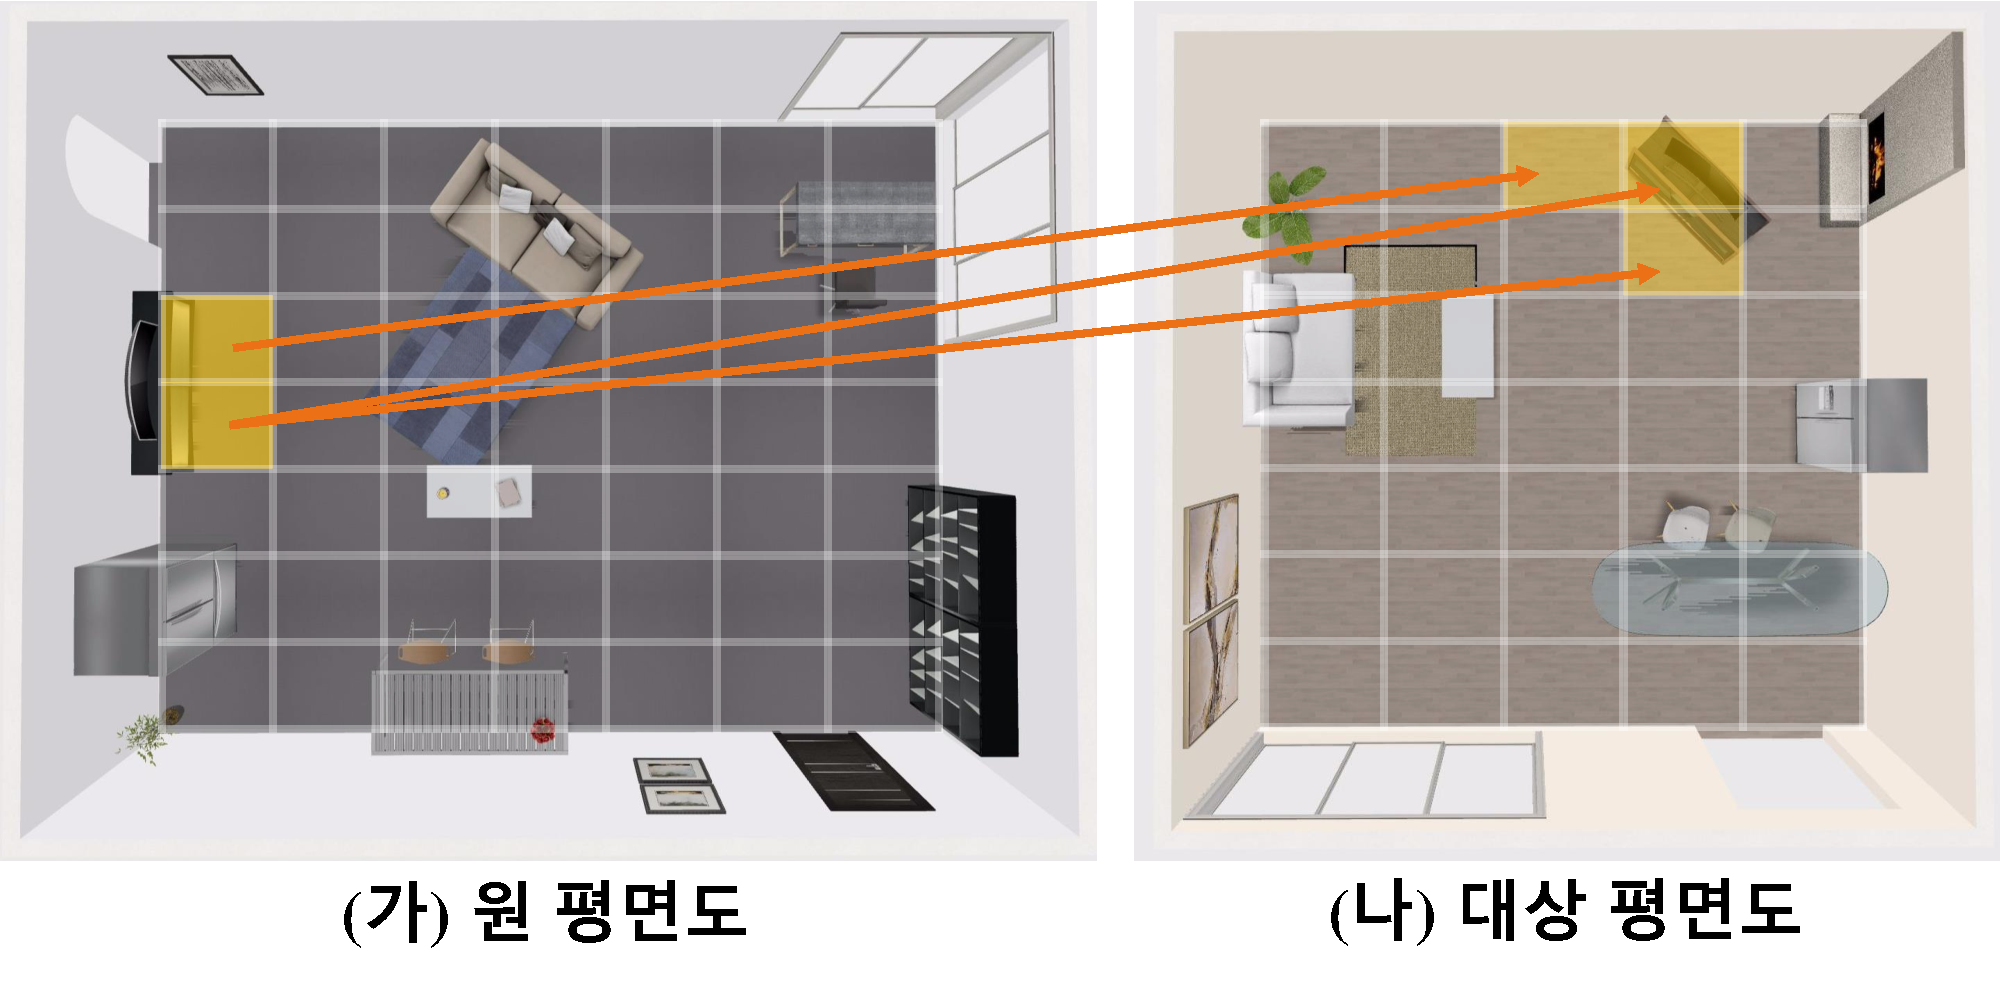
\includegraphics[width=15cm]{images/mapping.pdf}
\caption{평면도 쌍의 공간 매핑}
\label{fig:mapping}
\end{figure}

%집안 공간 매핑 실험
본 연구에서는 사람들이 서로 다른 집 구조에서 의미적으로 유사한 위치를 판단하는 기준을 파악하기 위해 20명의 실험 참가자를 모집하여 실험을 진행하였다. 본 연구에서는 공개 평면도 저장소~\cite{floorplanner}를 활용하여 다양한 크기와 가구 배치를 지닌 20쌍의 평면도를 수집하였고, 각각의 평면도를 1제곱미터 크기의 정사각형 격자 형태로 쪼개었다. 각 평면도 쌍은 4-5명의 실험 참가자들에게 임의로 배정되었다. 참가자는 각 평면도 쌍에 대해, 한쪽 평면도의 격자 공간을 다른 평면도의 격자에 매핑하는 임무를 수행하였다 (그림 \ref{fig:mapping}). 그림에서 나타나는 것처럼 참가자들은 하나의 격자 공간을 여러 공간에 매핑할 수도 있는데, 이는 집이나 가구 크기의 차이로 인해 동일한 의미를 나타내는 격자의 개수가 달라질 수 있기 때문이다. 이 과정을 통해 총 2,921개의 레이블된 실측 자료(ground truth)를 획득하였다. 또한 참가자들과 짧게 인터뷰를 진행하여, 매핑 결과에 대한 이유와 생각을 얻고자 하였다.

%다양한 집 구조에 대해 사람이 인식하는 의미적으로 유사한 위치를 파악하기 위해, 우리는 20명의 실험 참가자를 모집하여 집안 공간에 대한 매핑 실험을 수행했다. 우리는 Floorplanner~\cite{floorplanner}와 같은 공개 평면도 저장소 등을 활용하여, 다양한 크기와 가구 배치를 지닌 20쌍의 각기 다른 평면도를 수집했다. 우리는 각각의 평면도를 1제곱미터 크기의 정사각형 격자 형태로 나누었다. 각 참가자들은 평면도 A의 각 격자에 대해, 평면도 B에서 가장 의미적으로 유사한 격자를 찾는 일을 수행했다. 각각의 평면도 쌍은 4~5명의 실험 참가자들에게 임의로 배정되었다. 참가자들은 그림 \sclee{그림}에서와 같이 일대다 매핑을 수행할 수 있었는데, 이는 작은 평면도에서 한 격자가 큰 평면도에서는 여러 격자에 걸쳐서 같은 의미를 지닐 수 있기 때문이다. 이 과정을 통해 우리는 총 2,921개의 레이블된 ground truth를 획득하였다. 또한 참가자들과 짧은 인터뷰를 진행하여 그들의 매핑 결과에 대한 이유를 얻고자 하였다.

\begin{figure}
\centering
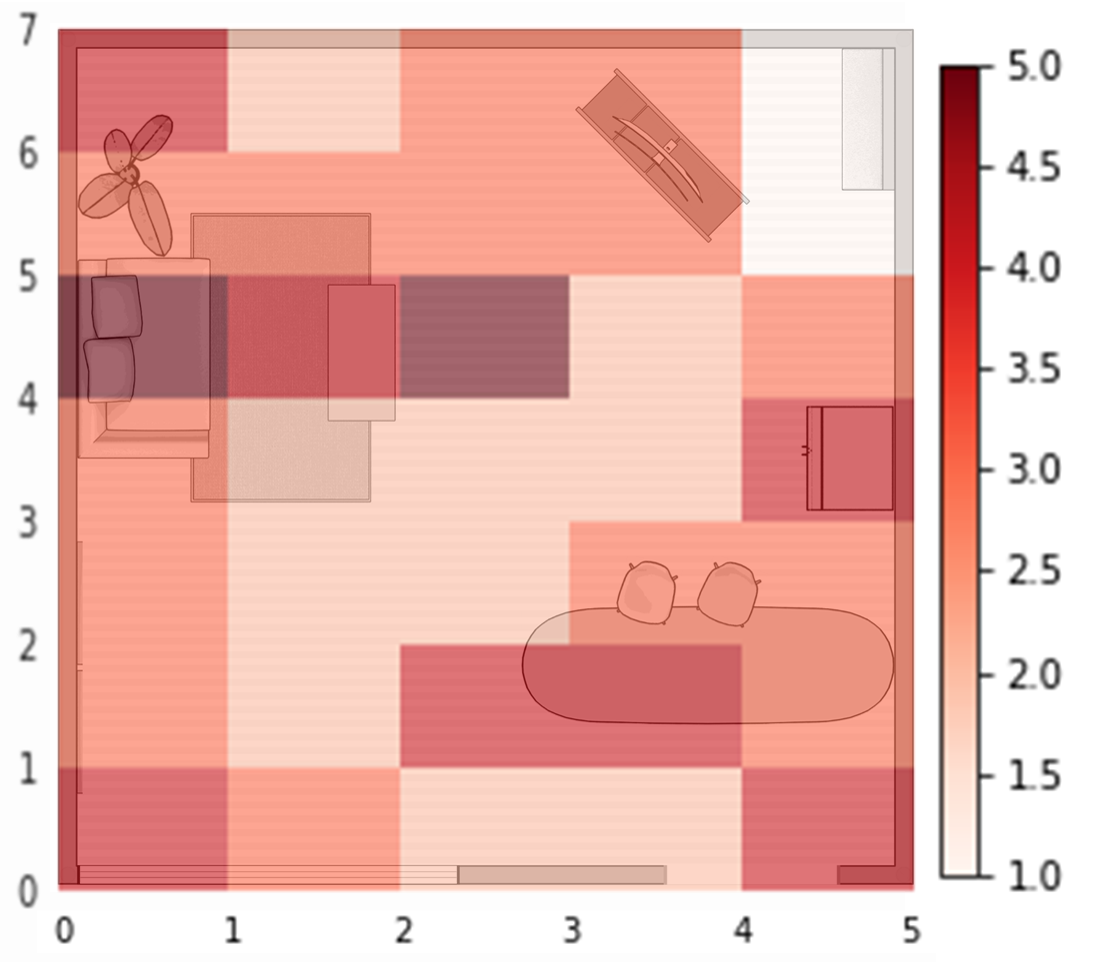
\includegraphics[width=10cm]{images/heatmap.png}
\caption{매핑 일치도 히트맵}
\label{fig:heatmap}
\end{figure}

참가자는 대부분 집안 가구와 가까운 격자에서부터 매핑을 시작했다. 그 후 가구와 가구 사이를 오가는 경로를 상상하면서 나머지 격자를 매핑했다. 그림 \ref{fig:heatmap}는 평면도 하나에 대한 매핑 결과를 표현한 히트맵으로, 참가자들의 매핑이 서로 얼마나 일치하였는지를 보여준다. 예를 들어, 소파에 해당하는 격자는 모든 참가자가 동일한 격자로 매핑을 이은 반면, 아무런 가구가 배치되지 않은 TV 뒤 구석 위치는 그 어떤 참가자도 동일한 격자로 매핑하지 않았다. 이는 사람들이 의미적으로 유사한 공간을 집안 가구와 연결지어 생각하는 경향이 있음을 내포한다.
\sclee{뭔가 수치가 있었으면 좋겠다. e.g., 가구와 바로 근처 격자의 평균 일치도 vs. 나머지 격자의 평균 일치도}

관찰 결과는 `의미적으로 유사한 공간'을 집안 가구를 중심으로 정의할 수 있는 뒷받침이 된다. 나의 집안에서의 상황과 행동은 내가 사용 중인 집안 가구(냉장고, 식탁 등)와 연관성이 있다. 내가 특정 가구에 가까이 서서 이를 바라보고 있다는 것은 내가 가구와 인터랙션을 하고 있다는 강한 지표가 되며, 이는 \cite{philipose2004inferring}의 연구 결과와도 일치한다. 나의 집안 특정 위치에 대해, 상대방의 집에서 의미적으로 유사한 공간은 동일하거나 유사한 목적을 수행하는 공간, 혹은 그러한 가구 근처의 공간이 된다. 같은 측면에서, 의미적으로 유사한 방향 역시 `TV를 보고 있다'와 같이 목적과 역할이 동일하게 나타나는 방향으로 나타날 수 있다.

% 의미적으로 유사한 위치를 찾는 방법 탐구
%heterogeneous floor plan
% 서로 다른 집의 구조를 맵핑하는 방법 탐구
% 맵핑이 필요하다는 것.
% 사람들 모아서 스터디 해봤다는 것.
% 결과
% 이 관점에서 바라보는 방향도 '선상에서 가장 가까이 위치한 가구'로 표현할 수 있겠더라.

\section{\sysname\ 아키텍쳐}

% \sysname을 만들었다!
\woinjung{다시 쓴 문단: `비슷한 장르'의 의미를 명확히 하려 함. 이 섹션이 보여주는 것이 플랫폼과는 거리가 먼 것 같아서 플랫폼이라는 표현은 없앴음. }
\sysname\은 아바타 로봇, 사용자 및 아바타 위치 인식 모듈, 의미적 위치 변환 모듈, 아바타 구동 모듈로 구성된다. \highlight{이 모듈들은 향후 텔레프리즌스 로봇에 기반한 \concept\를 제공하는 서비스 개발에 공통적으로 요구되는 핵심적 요소들이다.} 아래는 각 모듈들에 대한 설명이다.

%\sysname\은  (1) 사용자의 집안의 위치를 인식하고, (2) 상대방측 로봇이 '의미적으로 동일한 위치'로 (3) 이동하도록 조종하는 모듈들로 구성된다.

%\sysname\은 아바타 로봇과, 사람의 집안 위치를 인식하고, 의미적으로 동일한 위치를 찾고, 로봇을 조종하는 모듈로 구성된다. \highlight{위 모듈들은 비슷한 장르의 어플리케이션을 개발하는 데 있어 공통적으로 요구되는 핵심적인 요소들로, 향후 \concept\를 제공할 수 있는 다른 기술들을 탐구하는 데 있어 공통의 플랫폼으로 작동할 수 있을 것이라 생각한다.} 아래는 각 모듈들에 대한 설명이다.

%%%%%%%%%% 생각들 %%%%%%%%%%
% 각 모듈의 설명에서 넣어야 하는 내용은 무엇일까?
% - 각 모듈의 requirement
% - 각 모듈의 구현에서 중요하게 생각해야하는 요소들
%%%%%%%%%%%%%%%%%%%%%%%%%%

%\wonjung{아래 서브섹션들이 각 모듈의 requirement} 
\subsection{아바타 로봇}
% 사람이 인식하는 외형
\wonjung{이 문단은 무엇을 말하려는지 잘 모르겠음. '로봇은 상대방 아바타의 물리적 형체이다.'를 말하려고 하는 건가? 그렇다면 로봇의 물리적 형태가 어떻게 되어야 한다는 요구 조건도 이야기해야하지 않나? } 
아바타 로봇의 선택은 실제 사람에게 인식되는 형체를 결정한다. 이는 시각적인 요소 뿐만 아니라 촉각, 청각적인 요소를 모두 포함한다. 로봇에 디스플레이가 달려있다면 무엇을 보여줄 것인지, 스피커가 달려있다면 어떤 소리를 들려줄 것인지, 로봇을 건드렸을 때 어떤 느낌이 드는지 등의 요소가 아바타 로봇이 어떻게 느껴지는 지에 영향을 준다.

% 실제 시스템이 해결해야 하는 여러 문제를 던져줌.
\wonjung{고쳐써보았는데, 맨 마지막 문장은 실체가 뭔지 모르겠어서 그대로 둠. }
선택한 아바타 로봇의 성능은 시스템 구현의 여러가지 제약사항으로 작용한다. 아바타 로봇의 배터리 용량은 시스템의 구동시간에 영향을 주며, 로봇이 이동 속도는 상대방의 움직임 속도 재현에의 제약이 된다. 또한 생활 환경 공간에는 물리적 장애물들이 존재할 수 있다. 로봇의 형태 및 구동의 안정성에 따라 적용 가능한 환경에 제약이 생길 수 있다.
%또한 선택한 아바타 로봇의 성능은 실제 시스템 구현 측면에서 여러가지 문제를 던져준다. 아바타 로봇의 배터리 성능은 시스템의 구동시간에 영향을 주며, 로봇이 움직이는 속도는 사람의 움직임을 재현하는 데 있어 제약을 준다. 또한 실제 생활 환경에서는 바닥에 장애물들이 있을 수 있으며, 로봇의 형태 및 구동의 안정성에 따라 적용 가능한 환경에 제약이 생길 수 있다.

\wonjung{위치가 가장 핵심적 정보라는 것의 근거가 있는지? 위치가 소리보다 중요하다는 주장할 수 있는지?  마지막 문장은 아래 모듈의 역할로 보이는데 왜 이 서브섹션에 포함되 있는지 모르겠음. }
\subsection{사람 및 아바타의 집안 위치 인식 모듈}
\sysname\이 \concept\ 전달을 위해 가장 핵심적으로 인식해야 하는 정보는 사용자의 위치이다. 사용자 위치 인식은 사용자에게 장치 착용 없이 이루어져야 한다. \ref{sec:design_workshop} 장에서 논의했듯, 일상생활 중 지속적으로 장치를 착용하도록 하는 것은 사용자에게 상당한 불편함을 주기 때문이다. 또한 이 모듈은 사용자의 물리적 위치를 집 공간 내 사물들의 배치에 연결지어 의미적 위치로 변환할 수 있어야 한다. 

%\sysname\이 \concept\ 전달을 위해 가장 핵심적으로 인식해야 하는 정보는 사람의 위치다. 해당 모듈은 \ref{sec:design_workshop} 장에서 얘기했듯이 사람에게 특별한 장비 착용을 요구해서는 안된다. 또한 인식된 위치는 집안 가구들의 위치와 관계맺어 해석될 수 있어야 한다. \yjc{내용 추가 필요}
%사용자 위치 인식에  \ref{sec:design_workshop} 장에서 논의했듯이 사용자에게 장치 착용을 요구해서는 안된다. 또한 인식된 위치는 집안 가구들의 위치와 관계맺어 해석될 수 있어야 한다. \yjc{내용 추가 필요}


\wonjung{'삶의 방식'이라는 단어가 혼동스러움. '의미적 위치 변환'에 필요한 개념이 아니면 쓰지 않는 것이 명확해 보임.  }
\subsection{의미적 위치 변환 모듈}
위 모듈에서 인식한 물리적 위치 값은 의미적 위치 변환 모듈로 전달된다. 이 모듈은 시스템이 연결하는 두 집의 물리적 위치를 의미적 유사성을 이용하여 매핑(mapping)하여준다. 두 집의 물리적 형태에 차이가 있더라도, 로봇이 의미적으로 유사한 곳에 위치하도록 하여 \concept\을 느끼도록 한다. 

%위 모듈에서 인식한 물리적 위치 정보는 의미적 위치 변환 모듈로 전달된다. 이 모듈이 가장 핵심적으로 다루는 문제는 `집의 형태가 서로 다르다'는 문제다. 집의 형태, 삶의 방식에 따라 특정 위치에서 맥락이 다르게 형성되기에 두 집 사이에 맥락을 동기화 시키기 위해서는 가장 유사한 의미적 위치를 찾는 모듈이 핵심적이다. \yjc{내용 추가 필요}
%위 물리적 위치 인식 모듈에서 인식된 정보는 이후 의미적 위치 변환 모듈로 전달된다. 이 모듈에서 가장 핵심적으로 해결하는 문제는 `집의 형태가 서로 다르다'는 문제다. 집의 형태, 삶의 방식에 따라 특정 위치에서 맥락이 다르게 형성되기에 두 집 사이에 맥락을 동기화 시키기 위해서는 가장 유사한 의미적 위치를 찾는 모듈이 핵심적이다. \yjc{내용 추가 필요}

\subsection{아바타 구동 모듈}
의미적 변환 모듈을 통해 의미적인 동기화 후에는, 아바타 구동 모듈이 실제 로봇을 목표 위치로 이동시킨다. 해당 모듈은 아바타 로봇과 실제 인간 움직임 간의 차이를 최소화시켜야 한다. \yjc{내용 추가 필요}

%변환 모듈을 통해 의미적인 동기화가 완료되면, 아바타 구동 모듈이 실제 로봇을 구동한다. 해당 모듈은 아바타 로봇과 실제 인간 움직임 간의 차이를 최소화시켜야 한다. \yjc{내용 추가 필요}


%%%%%%%%%%%%%%%%%%%%%%%%%%%%%%%%%%%%%%%%%%%%%%%%%%%%%%%%%%%%%%%%%%%%%%%%%
\begin{figure}
\centering
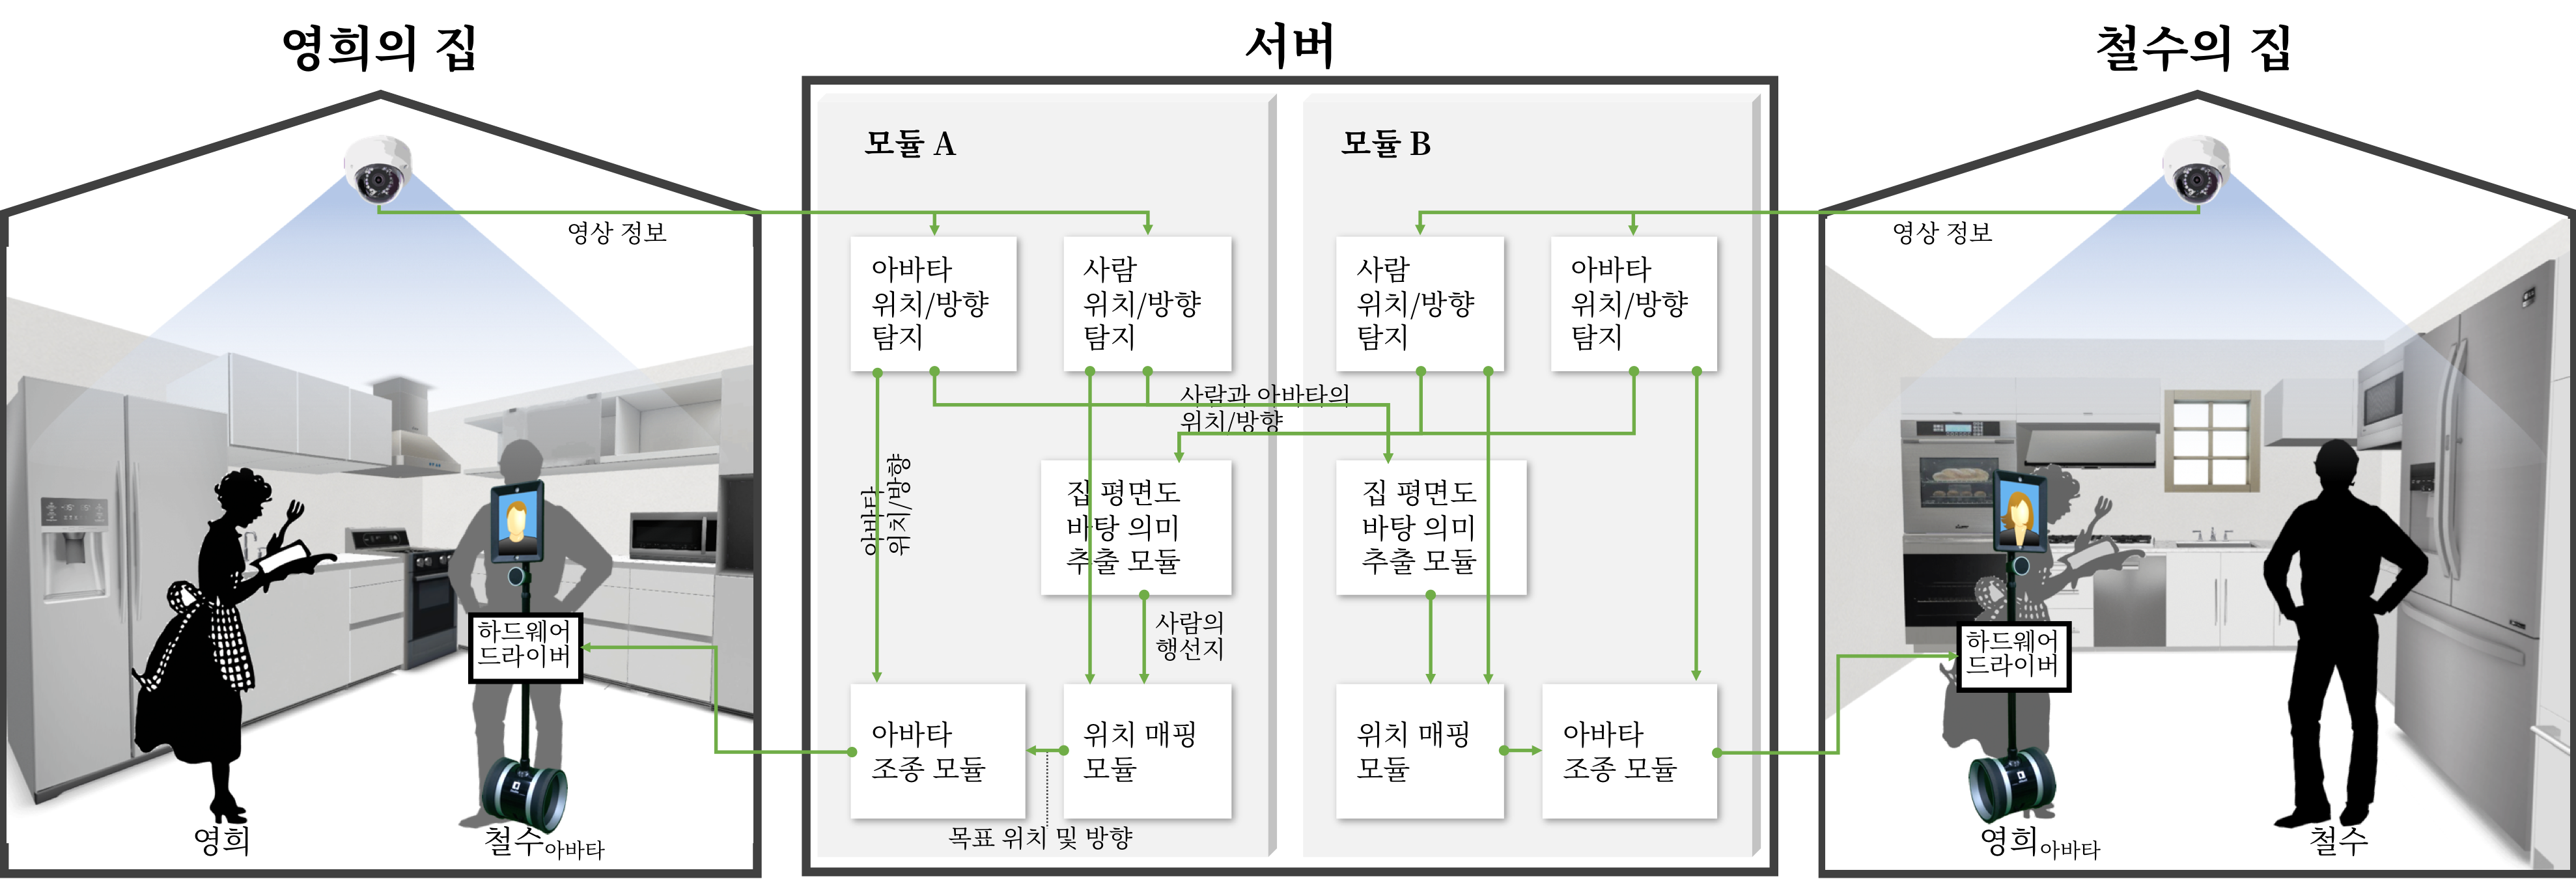
\includegraphics[width=0.95\textwidth]{images/architecture}
\caption{\sysname\ 아키텍쳐 모식도}
\label{fig:architecture}
\end{figure}
%%%%%%%%%%%%%%%%%%%%%%%%%%%%%%%%%%%%%%%%%%%%%%%%%%%%%%%%%%%%%%%%%%%%%%%%%

\
\section{\sysname의 기술적 구현}
\label{sec:system_implementation}
위에서 제시한 아키텍쳐의 기술적인 구현은 \cite{kang2018homemeld}에서 더 자세히 다루어졌다. 본 논문에서는 해당 아키텍쳐 구현의 핵심 아이디어, 텔리프레즌스 로봇과 의미적으로 유사한 위치 매핑이 어떻게 \concept\ 형성에 영향을 끼치는지 확인하는 데 집중한다.

%위에서 제시한 아키텍쳐의 기술적인 구현은 \cite{kang2018homemeld}에서 집중적으로 다루어졌다. 본 논문은 해당 아키텍쳐를 구현하는 데 있어 핵심적으로 제시한 두가지 접근, 텔리프레즌스 로봇과 의미적으로 유사한 위치가 어떻게 \concept\ 형성에 영향을 끼치는지 확인하는 데 집중한다.

본 논문에서는 \cite{kang2018homemeld}에서 제시한 \sysname\을 그대로 사용하지 않고, 핵심 모듈들을 인간 참여(Human-in-the-loop) 형태로 바꾸어서 오즈의 마법사(Wizard-of-Oz) 실험을 진행한다. 첫째, \cite{kang2018homemeld}의 구현체를 사용할 경우 실험 수행의 비용이 매우 커지기 때문이다. 사용자의  집안 위치 인식을 위해서는 각 사용자 별로 학습된 딥러닝 모델을 요구한다.해당 모델을 학습에는 고성능의 그래픽 카드 (Nvidia GeForce GTX TITAN X)를 이용할 경우에도 이틀 가량의 긴 시간이 필요하다. 따라서 \cite{kang2018homemeld}의 구현체는 다수의 커플을 대상으로 하고자 하는 본 연구의 실험에 적합치 않았다. 

\wonjung{둘째 이유와 마지막 이유의 차이를 모르겠음. '둘째'가 이유고 '마지막'이 해결방식인가? 일단 그렇게 생각하고 다시 써봄}
둘째로 \cite{kang2018homemeld}에서 다룬 기술적 문제들(서로 다른 집의 모양, 텔레프레즌스 로봇의 동작 제어 등)의 경우, 구현체의 시스템 동작 환경을 제한하는 것을 요구한다. 실험진행자가 로봇을 조종하는 방식으로 시스템을 제어할 경우, 더 다양한 상황(사람이 눕거나, 방 밖으로 나가는 상황 등)에 대처하여 실험을 진핼할 수 있다. 구체적인 실험 과정은 \ref{sec:userstudy} 장에서 서술한다.
%본 논문에서는 \cite{kang2018homemeld}에서 제시한 \sysname\을 그대로 사용하지 않고, 핵심 모듈들을 인간 참여(Human-in-the-loop) 형태로 바꾸어서 오즈의 마법사(Wizard-of-Oz) 실험을 진행한다. 첫째, \cite{kang2018homemeld}의 구현체의 경우 집안 위치 인식을 위해 커플에 맞추어 학습된 딥러닝 모델을 이용한다. 해당 모델을 학습하는 데는 고성능의 그래픽 카드 (Nvidia GeForce GTX TITAN X)를 이용할 시 이틀 정도의 시간이 필요하다. 이와 같은 시스템의 특성은 짧은 시간 안에 다양한 커플을 대상으로 하고자 하는 후술할 실험의 목표에 맞지 않았다. 둘째로 \cite{kang2018homemeld}에서 핵심적으로 해결한 문제들(서로 다른 집의 모양, 텔레프레즌스 로봇의 움직임 등)의 경우 특수한 실험 환경 디자인을 통해 효과적으로 제거할 수 있었다. 마지막으로 인간 참여형 시스템을 운용할 경우 사람이 눕거나, 방 밖으로 나가는 상정되지 않은 상황에서 \cite{kang2018homemeld}의 시스템보다 자연스럽게 대응할 수 있을 것으로 판단했다. 구체적인 실험 과정은 \ref{sec:userstudy} 장에서 서술한다.


\chapter{\expUser}
\label{sec:userstudy}

\ref{sec:design_workshop}장에서 우리는 `\concept'\를 전달하는 시스템 \sysname의 핵심 요소와 모듈들을 제시했다. 본 장에서는 \sysname\을 오즈의 마법사(Wizard-of-Oz) 형태로 사용자들에게 체험하도록 하여 그 효과를 관찰하고자 한다.

본 장은 다음과 같이 구성된다. 첫째, 시나리오 기반의 실험 설계 과정에 대해 이야기한다. \concept\를 체험할 수 있는 실험 환경 구성의 어려움과, 이를 실험 디자인 과정에서 다룬 방법을 서술한다. 둘째, 실험에 참여한 피험자 부부들의 특성에 대해 서술한다. 총 5팀, 10명의 사람들이 참여했으며, 이들 부부가 어떻게 평소에 시간을 같이 보내는지 얘기한다. 마지막으로 실험을 통해 관찰한 결과를 다룬다. \sysname\ 디자인 과정에서 고려한 요소들이 실제 사용자 실험에서 어떻게 나타났는지 얘기한다. 본 실험은 IRB 승인(KH2017-18) 아래 진행했다.


%%%%%%%%%%%%%%%%%%%%%%%%%%%%%%%%%%%%%%%%%%%%%%%%%%%%%%%%%%%%%%%%%%%%%%%%%
\begin{figure}
\begin{subfigure}{.5\textwidth}
  \centering
  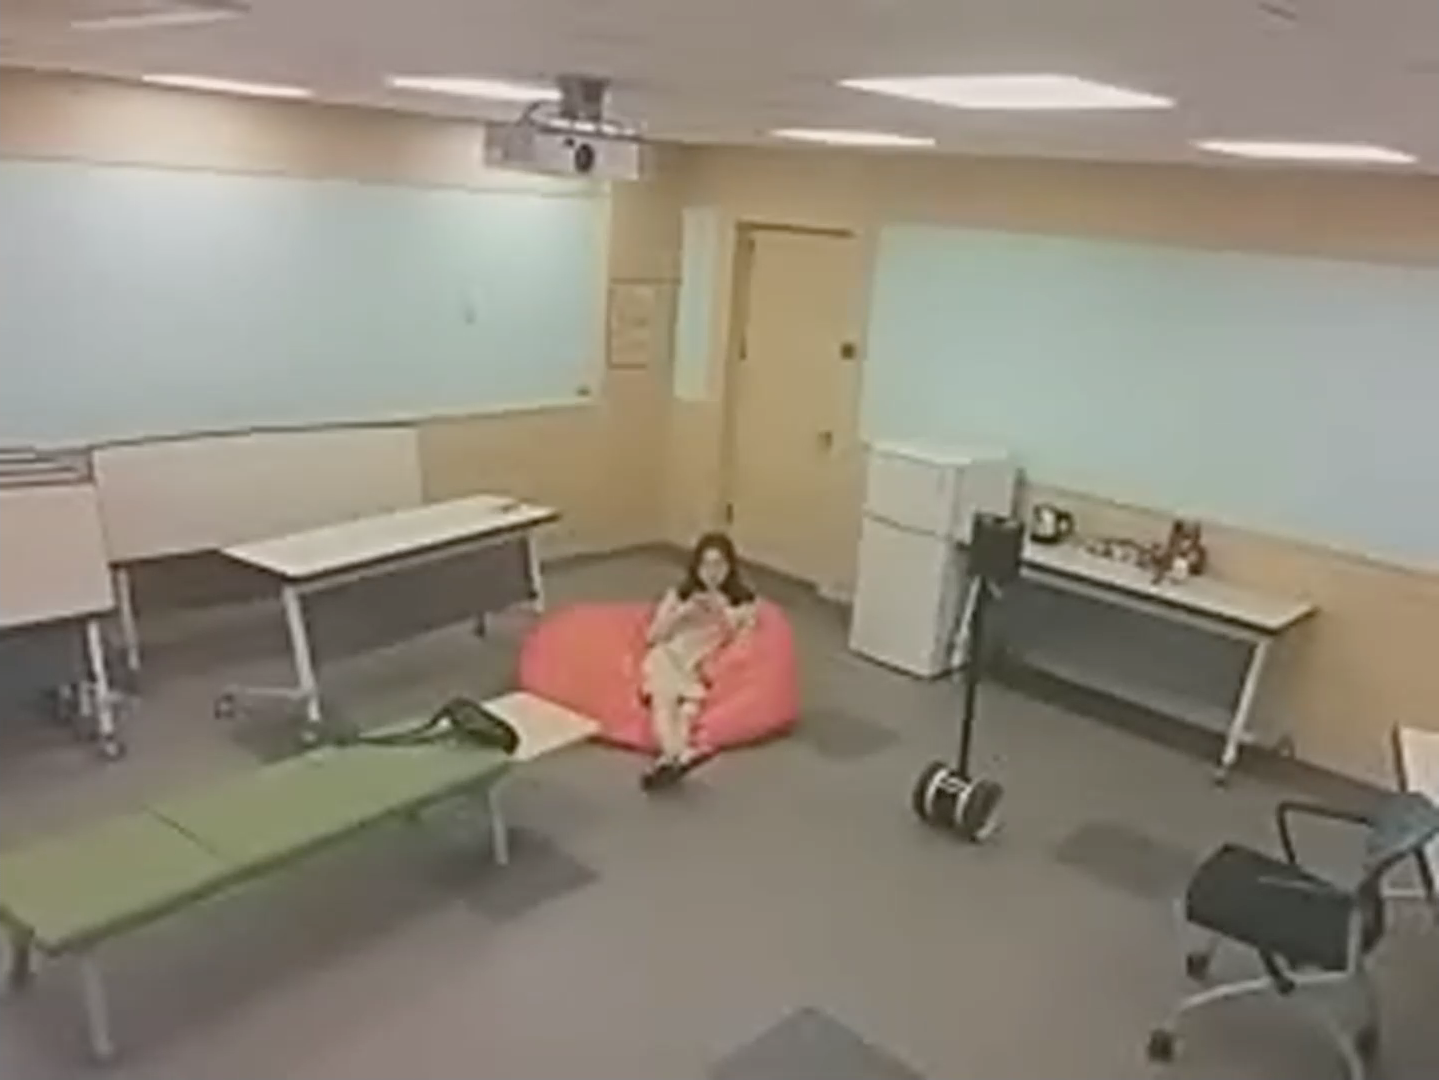
\includegraphics[width=0.9\textwidth]{images/sceneA}
\end{subfigure}
\begin{subfigure}{.5\textwidth}
  \centering
  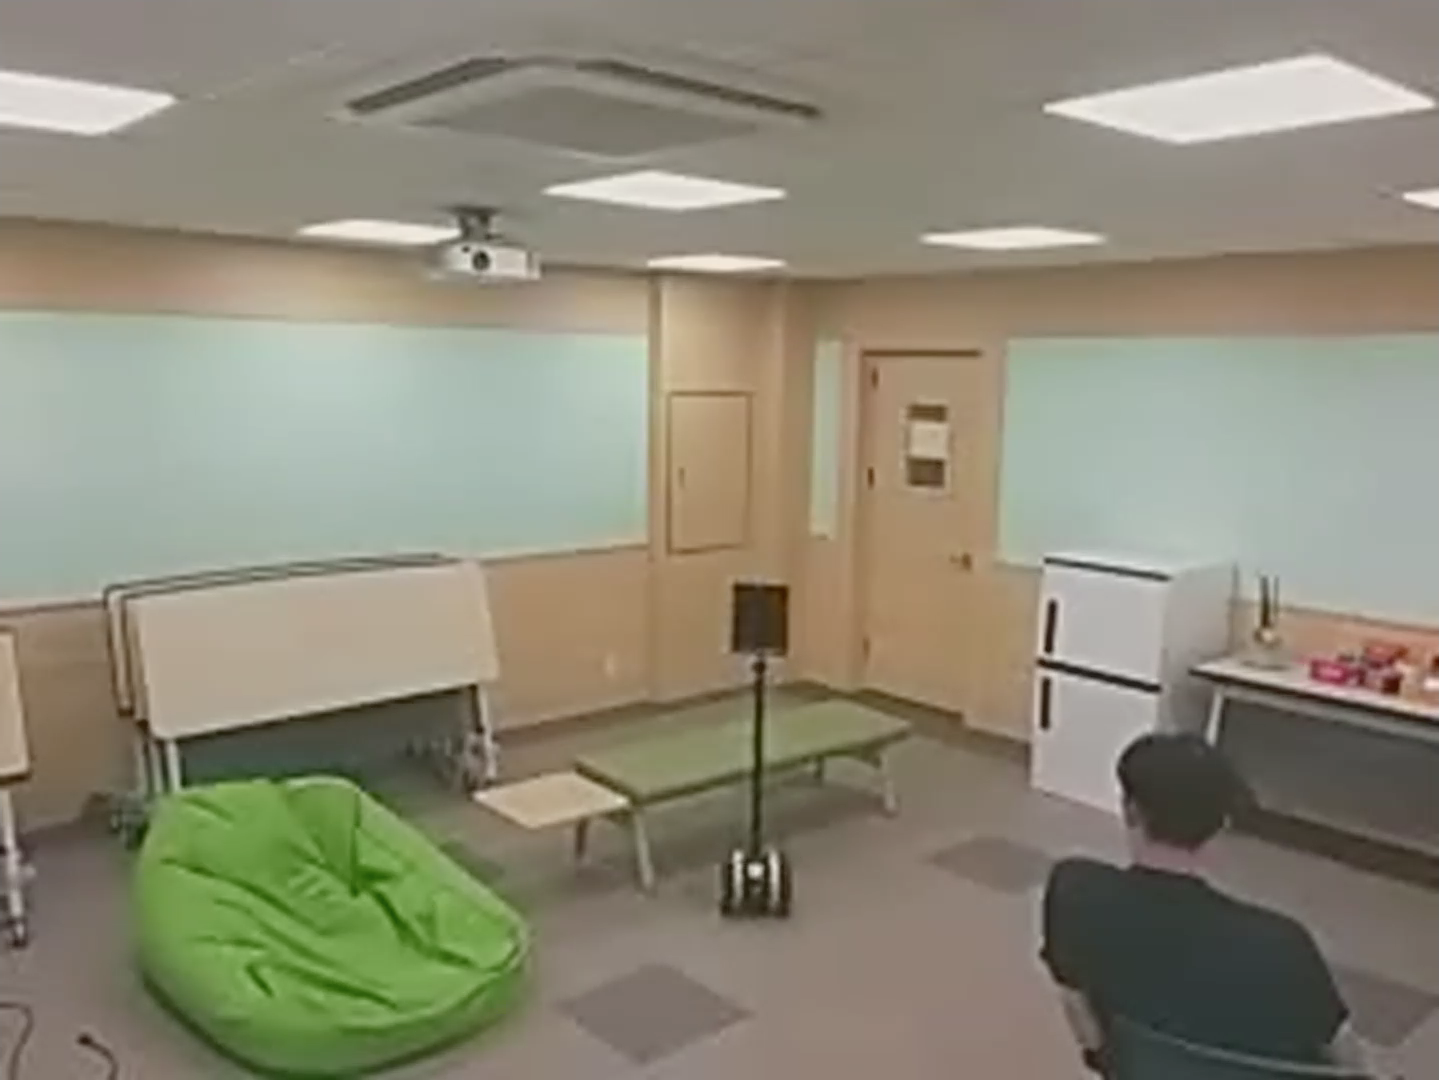
\includegraphics[width=0.9\textwidth]{images/sceneB}
\end{subfigure}
\caption{랩 환경에서 진행된 시나리오 중심 사용자 스터디 실험 장면}
         % 로봇 아바타는 상대방의 의미적 위치로 지속적으로 이동하며 두 방 사이를 연결짓는다.
\label{fig:userstudy_scene}
\end{figure}
%%%%%%%%%%%%%%%%%%%%%%%%%%%%%%%%%%%%%%%%%%%%%%%%%%%%%%%%%%%%%%%%%%%%%%%%%


\section{실험 디자인}

% 은근한 함께 삶의 섬세함
`\concept'\는 섬세한 감각이다. 일상 속, 익숙한 공간에서 시간을 함께 보낼 때 생겨나는 미묘한 감각을 실험 환경 속에서 포착하기 위해서는 실험 또한 섬세하게 디자인되어야 한다. 본 장에서는 \concept\를 실험하기 위한 디자인으로 \expUser\를 제시한다. 또한 섬세한 감각을 실험실 환경에서 재현하기 위해 어떠한 과정을 거쳤는지 서술한다.

\subsection{목표}
\label{subsec:exp_goal}

우리는 앞서 \ref{sec:concept}장에서 \concept\를 형성할 때 필요한 5가지 핵심 상태에 대해 얘기했다.

\begin{center}
\begin{minipage}{.6\textwidth}
\begin{enumerate}[label=\Roman*., noitemsep]
	\item 상대방이 나와 같은 공간에 있다고 인지할 수 있는 상태
	\item 상대방의 상황(상태)을 언제든지 파악할 수 있는 상태
	\item 상대방이 나를 의식한다는 것을 인지하고 있는 상태
	\item 언제든지 상대방과 소통할 수 있는 상태
	\item 서로의 활동을 방해하지 않고 있는 상태
\end{enumerate}
\end{minipage}
\end{center}

\noindent 본 실험의 목표는 우리가 제시하는 \sysname\이 위에 나열된 상태의 형성에 어떤 도움을 주는 지 확인하는 것이다. 실제 함께 살아가는 사람들 사이에서 \concept\가 어떠한 형태로 나타나는 지 확인하고, 해당 순간에 컴퓨터 기술이 어떻게 녹아들 수 있는 지 보이고자 했다.


\subsection{실험 방법}

% 실험 방법 Overview
실험은 사전 인터뷰, 시나리오 체험, 사후 인터뷰 순서로 수행하였다.
먼저 \concept\와 관련된 피험자들의 의견을 수집하기 위해 약하게 구조화된 인터뷰(Semi-structured Interview)를 수행했다. 인터뷰를 통해 커플의 인구학적 특성 및 실제 일상생활에서 \concept\를 느끼는 순간들에 관해 조사하였다.
실험참가자들은 이후 집안 환경을 모사하여 꾸민 방으로 이동했다. 참가자들은 시험 공부, 드라마 시청, 여행 계획 세우기 등 미리 준비해온 업무를 수행하며 일상적인 시간을 보냈다. 동시에 참가자들은 영상 통화 및 \sysname\을 통한 연결을 체험했다.
사후 인터뷰 세션은 시나리오 체험 시간 동안 관찰된 행동을 중심으로 진행했다. 각 연결 기술의 사용자 경험의 차이와 특이 행동에 대한 참여자의 주관적 해석을 중점적으로 조사하였다.
전체 실험은 이틀에 걸쳐서 이루어졌다. 각 실험은 1시간 40분에서 2시간 길이로 진행했다.

인터뷰 자료 분석은 실험 종료 후 진행했다. 실험 결과는 녹취록 및 영상 자료로 정리 된 후 공동 연구자들에 의해 여러 번 검토되었다. 이후, \ref{sec:concept} 장에서 언급한 테마를 기반으로 관찰 결과를 정리했다.


\subsubsection{실험 참가자 모집}

실험 참가자들은 대학교(KAIST)내 구성원 커뮤니티 웹사이트에 모집 광고를 게시하여 모집하였다. 총 7쌍의 커플이 지원했으며, 이들 중 나이와 부부 형태의 다양성을 고려하여 5쌍을 선택했다. 참가자의 직업의 경우 대학원생의 비율이 높았지만, 해당 직업군은 떨어져 사는 생활을 경험하는 비율이 높기에 초기 연구에 적합하다고 보았다. 실험 참가자들은 함께 살아온 시간이 3개월 이상인 그룹으로 제한하였다. \concept\를 느끼기 위해서는 서로의 생활에 대한 깊은 이해가 필수적이므로, 일정기간 이상의 시간을 함께 보내는 것이 필요하다고 고려하였다. 총 10명의 실험 참가자에 관한 정보는 표 \ref{tab:userstudy_participants}에 정리되어 있다.


%%%%%%%%%%%%%%%%%%%%%%%%%%%%%%%%%%%%%%%%%%%%%%%%%%%%%%%%%%%%%%%%%%%%%%%%%
\begin{table}
\centering
\caption{\expUser\ 참여자 정보}
\label{tab:userstudy_participants}
\begin{tabu}{ccccc}
	\toprule
	\rowfont[c]{\bfseries}
	커플 & 나이 (성별) & 부부 형태 & 함께 산 기간 & 직업 \\
	\midrule
	가 & 27(남), 27(여) & 주말 부부		& 1년		& 대학원생 (둘다)	\\
	나 & 34(남), 31(여) & 주말 부부		& 3개월		& 대학원생, 직장인	\\
	다 & 33(남), 26(여) & 함께 사는 부부	& 1년 4개월	& 대학원생, 휴학중	\\
	라 & 29(남), 25(여) & 장거리 커플	& - 			& 대학원생, 직장인	\\
	마 & 32(남), 33(여) & 함께 사는 부부	& 1년 2개월	& 대학원생, 직장인	\\
	\bottomrule
\end{tabu}
\end{table}
%%%%%%%%%%%%%%%%%%%%%%%%%%%%%%%%%%%%%%%%%%%%%%%%%%%%%%%%%%%%%%%%%%%%%%%%%


% 왜 학교 커뮤니티에서 모집했지? - 고학력자 비중이 높지만, 초기연구에는 적합
% 왜 학교로 데려와서 인터뷰했지? - 이거는 얘기할 필요 없을 듯


\subsubsection{장소 구성}

% 핵심 포인트 => 장소를 만들 때 각 위치가 의미를 가질 수 있도록 잘 설계했다.

실험 장소는 학교 내에 서로 붙어 있는 3개의 세미나실을 이용해 구성했다. 첫번째 방에서는 인터뷰를 진행했으며, 나머지 두개의 방에 시나리오 체험을 위해 떨어져 있는 두 개의 거실을 모사했다. 이하 각 방은 인터뷰 방과 실험 방 A, B로 부른다.

실험 방 A와 B를 만들 때 핵심적으로 고려한 요소는 방 안의 각 장소를 구획별로 나누어 특별한 의미를 가지도록 하는 것이다. 이는 \ref{sec:system_design}장에서 얘기한 의미적 위치 기반 동기화의 효과를 최대화하기 위한 목적으로, 방의 각 면에 특정 목적에 맞는 가구들을 놓았다. 구성된 공간의 평면도는 그림 \ref{fig:floorplan}과 같다. 해당 그림을 기준으로, 북쪽에는 책상과 같이 공부와 관련된 가구와 TV를, 동쪽에는 잡동사니가 수납되어 있는 서랍을, 남쪽에는 편하게 쉴 수 있는 벤치와 빈백(bean bag)을, 마지막으로 서쪽에는 음식과 관련된 냉장고와 식료품 책상을 배치했다. 가운데 영역은 로봇이 자유롭게 움직일 수 있도록 비워 두었다. 위와 같이 가구들이 벽면에 붙어서 위치한 형태는 원룸형 스튜디오 아파트에서 매우 흔하게 발견할 수 있는 구조로, 스튜디오 아파트의 인테리어 사진을 참조해서 배치했다. 4면의 가구들의 경우, 흔히 검색되는 원룸 가구들 중 침대를 제외하고 주변에서 구할 수 있는 것들로 선택했다. 참고로 그림 기준 동쪽 면은 커다란 창문으로, 특정 의미적 위치로 구성하는 데 있어 일반적인 벽에 비해 어려움이 있었다. 이에 따라 다른 가구에 비해 의미 효과가 적은 수납 공간을 해당 면에 놓았다. 이 외 녹화 및 로봇 조종을 위해 TV 위쪽에 카메라를 각 실험방마다 두대씩 설치했다.

두 개의 실험방은 구성을 동일하게 맞추었다. 서로 다른 구성의 방으로 실험 환경을 구성할 경우, 두 실험방 각각에 대해 실험 참가자의 학습이 필요하고, 시스템 운용 시 위치 매핑이 필요하기에, \sysname\ 시스템의 본질적인 효과를 명확히 보기 위해서는 복잡한 요소는 통제하는 것이 더 낫다고 판단했다.


%%%%%%%%%%%%%%%%%%%%%%%%%%%%%%%%%%%%%%%%%%%%%%%%%%%%%%%%%%%%%%%%%%%%%%%%%
\begin{figure}
\centering
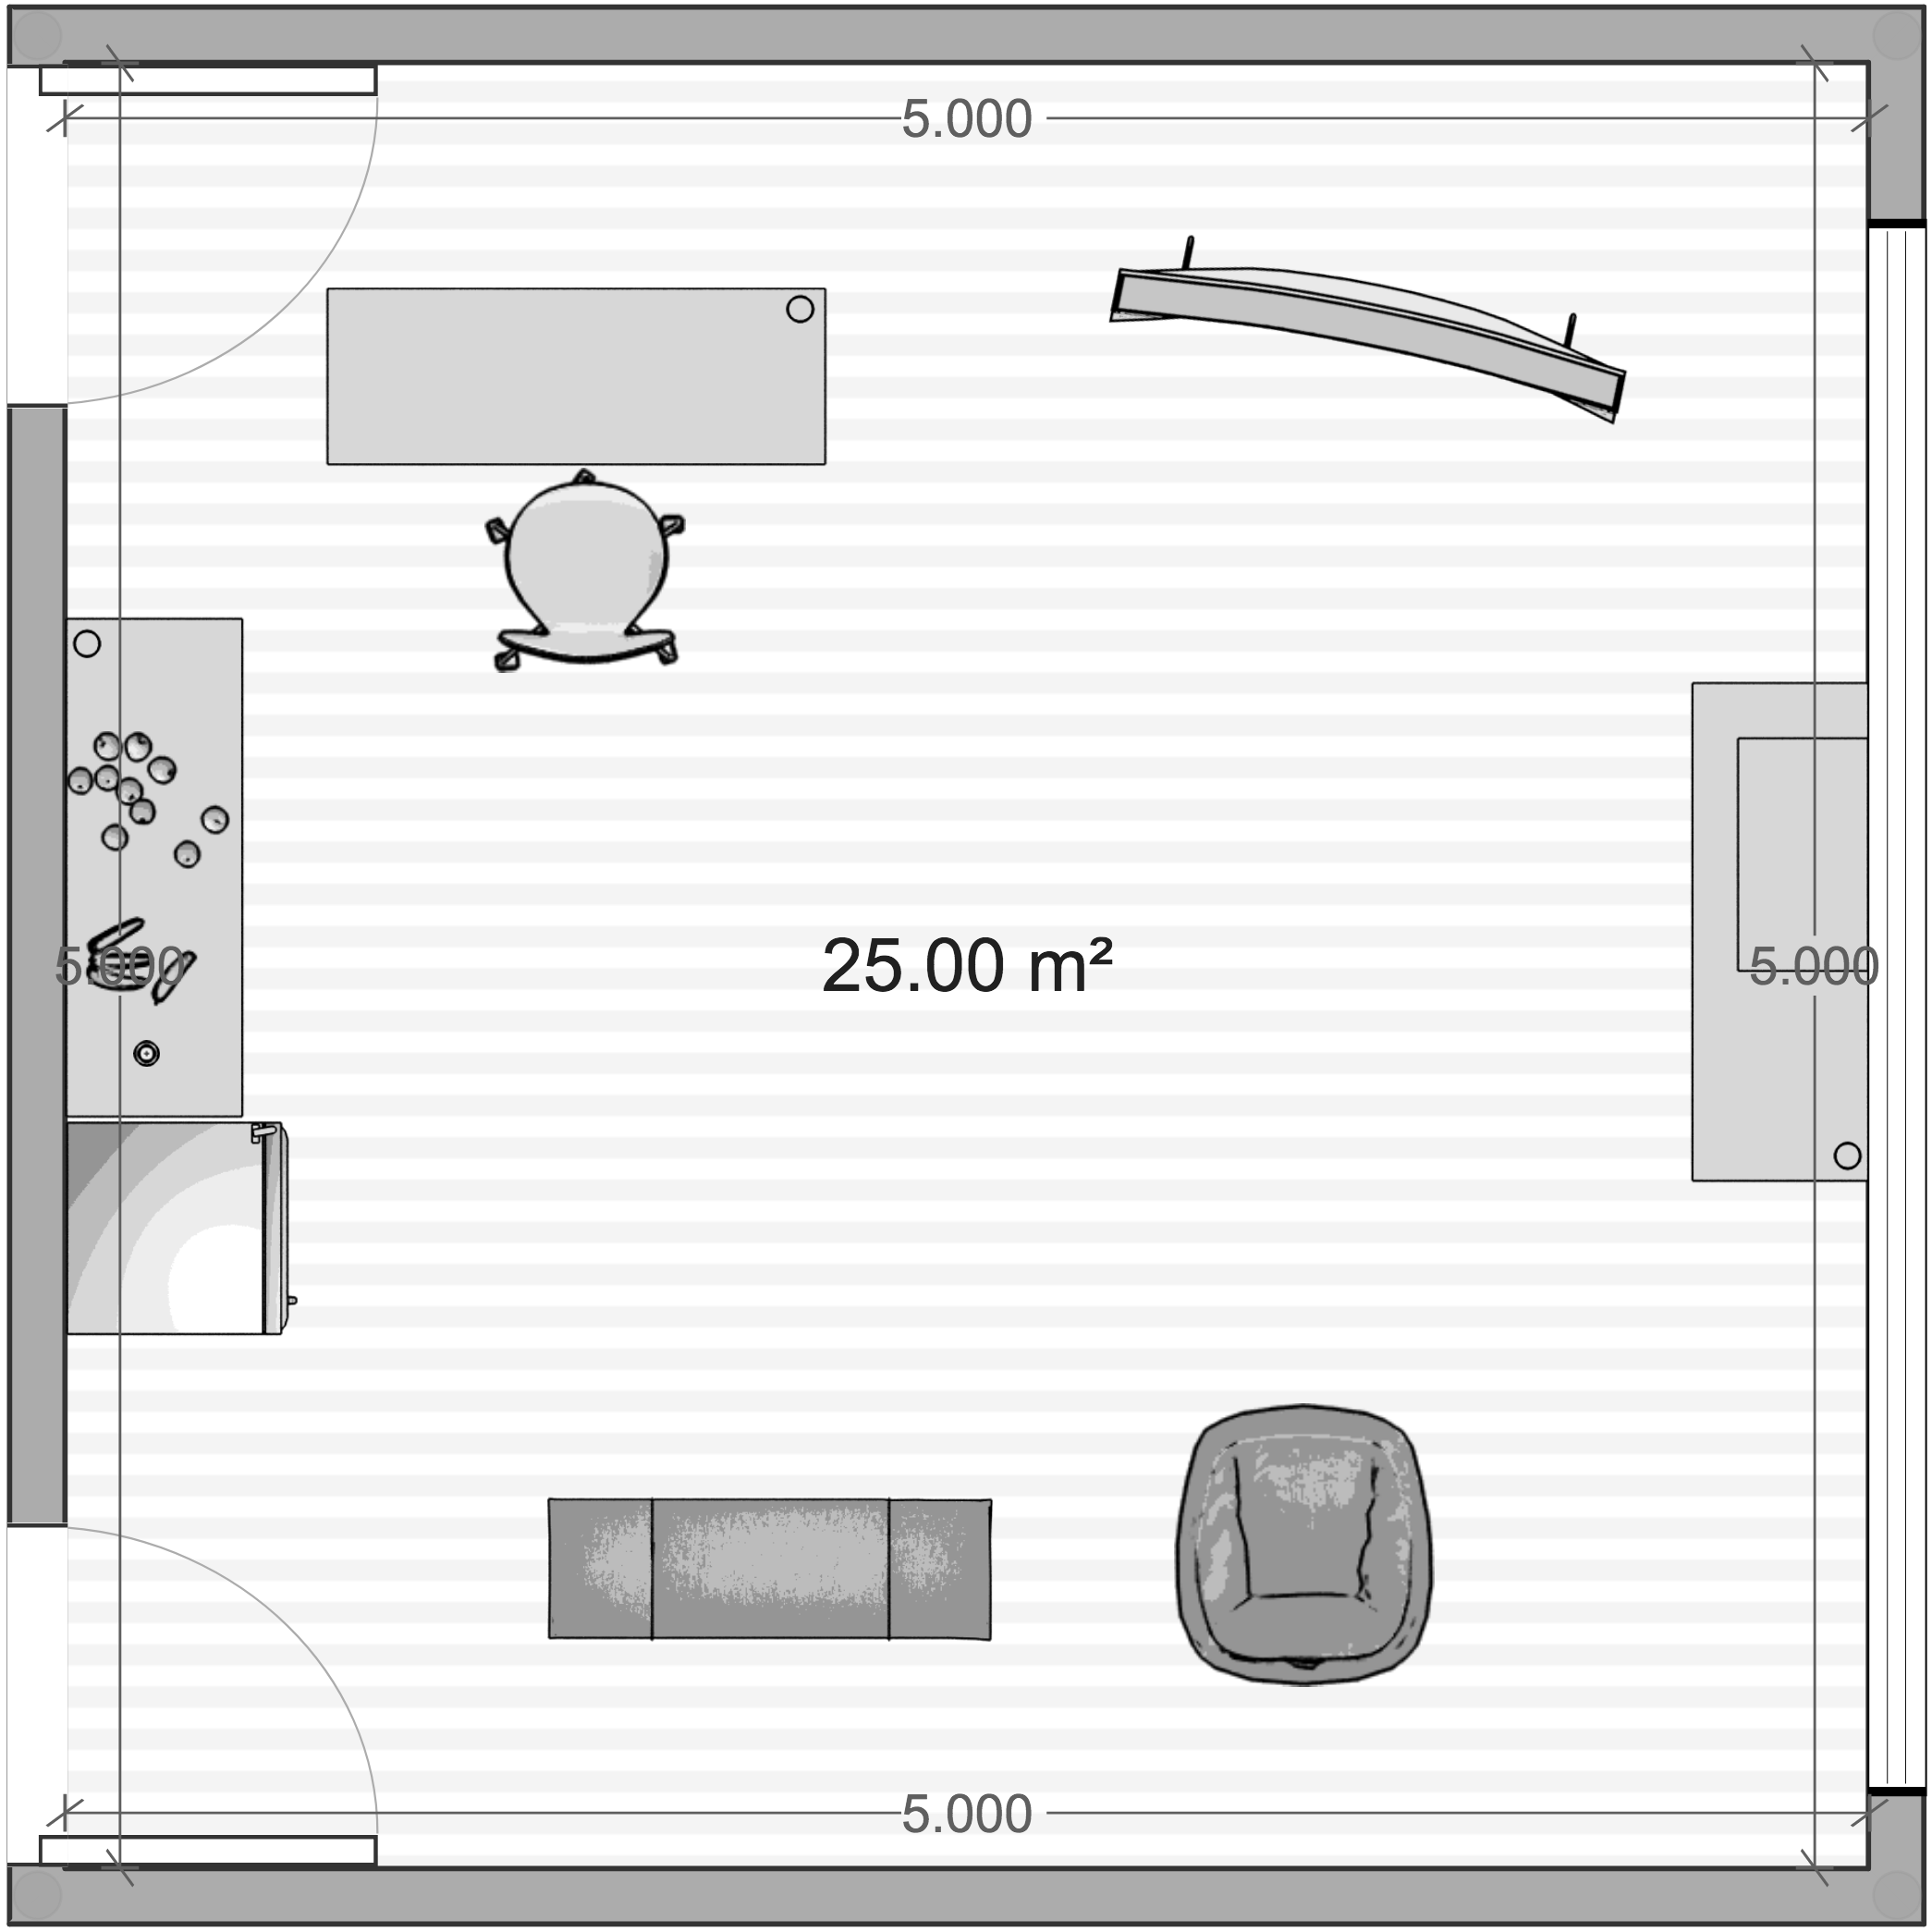
\includegraphics[width=0.6\textwidth]{images/floorplan}
\caption{집안 거실을 모사한 실험 장소의 평면도}
\label{fig:floorplan}
\end{figure}
%%%%%%%%%%%%%%%%%%%%%%%%%%%%%%%%%%%%%%%%%%%%%%%%%%%%%%%%%%%%%%%%%%%%%%%%%


\subsubsection{인간참여형 \sysname\ 시스템}

본 사용자 스터디에서는 \ref{sec:system_implementation}에서 언급했듯이 \cite{kang2018homemeld}에서 제시한 \sysname\을 인간 참여(Human-in-the-loop) 형태로 바꾸어서 오즈의 마법사(Wizard-of-Oz) 실험을 진행했다.

실험을 위해 텔레프레즌스 로봇의\cite{double_robotics} 조종 경험이 있는 두명의 조종사를 모집했다. 먼저 각 방에 설치된 스마트폰을 통해 각 방에 어디에 사람이 위치하는 지 영상을 관찰했다. 이후 각 조종사는 텔레프레즌스 로봇 조종 프로그램을\cite{double_drive} 통해 각 로봇을 동일한 위치로 움직였다. 로봇의 방향의 경우 상대방을 바라보고 있는 지 여부를 동기화하는 데 집중했다.

텔레프레즌스 로봇 사이는 음성 통화(FaceTime)로 연결하여 서로의 목소리 및 생활 속 일상 소음이 서로 전달 될 수 있도록 했다. 텔레프레즌스 로봇의 화면은 사용하지 않았다. 방향이 제대로 맞지 않으면 의미 있는 정보 전달이 이루어지지 않고, 로봇을 따라다니면서 화면을 보는 경우를 막기 위하여 화면은 띄우지 않는 방향으로 통제하기로 결정했다.


\subsubsection{사전 인터뷰}

사전 인터뷰는 커플의 인구학적 특성과 함께함의 형태 및 경험의 깊이에 대한 질문으로, 시스템 체험 전에 30분 동안 진행했다. 인터뷰에서 물어본 핵심 질문들은 다음과 같다. ``두 사람은 얼마나 오래 알고 지냈나요?'', ``함께 살기 시작하고 나서 상대방에 대해 더 잘 이해하게 되었다고 생각하시나요?'', ``평소에 집에 두 분이 함께 계시는 시간은 어느정도 되나요?'', ``같이 계실때면 두 분은 서로 어떻게 시간을 보내시나요?'', ``상대방이 피곤하다고 느끼신 적이 있나요?''. 자세한 핵심 질문 목록은 표 \ref{tab:userstudy_pre_questionnaire}에 나열했다.


%%%%%%%%%%%%%%%%%%%%%%%%%%%%%%%%%%%%%%%%%%%%%%%%%%%%%%%%%%%%%%%%%%%%%%%%%
\begin{table}
	\centering
	\caption{사전 인터뷰 핵심 질문 목록}
	\label{tab:userstudy_pre_questionnaire}
	\newcommand{\mr}[2]{\multirow{#1}{*}{#2}}
	\begin{tabular}{ll}
		\toprule
		\textbf{주제 (Theme)} & \textbf{종자 질문 (Seed Questions)} \\
		\midrule
		\mr{3}{``함께 삶''의 깊이}
		& 두 사람은 얼마나 오래 알고 지냈나요? \\
		& 함께 살고 있다는 확연히 느낀 순간이 있나요? \\
		& 함께 살기 시작하고 나서 상대방에 대해 더 잘 이해하게 되었다고 생각하시나요? \\
		\midrule
		\mr{2}{``함께 삶''의 형태}
		& 평소에 집에 두 분이 함께 계시는 시간은 어느정도 되나요? (주말 / 주중) \\
		& 같이 계실때면 두 분은 서로 어떻게 시간을 보내시나요? \\
		\midrule
		\mr{5}{``함께 삶''의 요소}
		& 함께 있을 때 아직 서로가 신경쓰이시나요? \\
		& 상대방이 피곤하다고 느끼신 적이 있나요? \\
		& 배려 받고 있다고 느끼신 적이 있나요? \\
		& 보통 대화를 어떻게 시작하시나요? \\
		& 말을 하지 않아도 함께 하실때는 서로의 기척을 잘 느끼시는 편인가요? \\
		\bottomrule
	\end{tabular}
\end{table}
%%%%%%%%%%%%%%%%%%%%%%%%%%%%%%%%%%%%%%%%%%%%%%%%%%%%%%%%%%%%%%%%%%%%%%%%%


\subsubsection{시나리오 체험}

시나리오 체험의 목적은 영상 통화 혹은 \sysname\이 제공되는 상황에서 \concept\가 어떻게 형성되는 지 참가자가 실제 체험해볼 수 있도록 하는 것이다. 그 과정을 돕기 위해 우리는 \concept\를 체험할 수 있는 적절한 시나리오를 제공하고자 했다.

시나리오 체험 세션은 15분의 길이를 가지는 3개의 세션으로 이루어졌다. 각 세션에서는 차례로, 서로 함께 있는 상황, 텔레프레즌스 로봇 아바타를 통해 소통하는 상황, 영상통화(Skype)를 통해 소통하는 상황을 체험했다. 자연스러운 환경을 위해 체험 중에는 실험 참여자들만 실험방에 위치하도록 했다. 연구자는 각 세션의 사이에 다음 실험을 위해 환경을 바꿀때만 출입하였다.

실험을 위한 시나리오를 기획하는 과정에서 가장 중요하게 고려한 요소는 어떻게 참가자들이 ``\concept''에 빠지도록 할 수 있을까였다. 우리는 두 사람이 조용한 환경에서 각자 자신의 할 일에 집중하고 있는 상황을 선택했다. 각자 할 일에 집중하고 있는 상황은 서로 대화가 잦지 않으며 서로 얼굴을 바라보지 않아도 괜찮다. 또한 주변 소리가 없는 고요한 환경에서 진행해도 어색함이 없으며, 움직임이 많지 않다. 이들 요소는 텔레프레즌스 로봇의 외형이 가지고 있는 여러 요소들의 영향을 통제할 수 있게 해주었다. 대면을 요구하지 않는 상황은 영상 통화의 필요성을 제거해 주었고, 배경 음악이 존재할 때 생기는 불편한 소음 또한 조용한 환경이기에 배제할 수 있었다.

실험 참가자들이 각자 할 일을 선정할 때는 다음과 같은 요소를 고려했다. (1) \textit{일상적이지만 명확한 할 일.} 실험 환경은 실제 살아가는 환경이 아니기에 일상적인 활동에 자연스럽게 빠져들기 힘들다. 이 문제를 해결하기 위해 우리는 실험 참가자들에게 미리 할 일을 들고 와달라고 부탁했다. 참가자들이 제시한 할일의 예시에는 시험 공부, 드라마 시청, 여행 계획 세우기 등이 있었다. (2) \textit{할 일의 집중도에 차이를 주기.} 두 사람에게 명확히 할 일을 정해주었을 때 두 사람 사이의 소통이 너무 적어지는 문제가 발견되었다. 집중도가 높아 소통의 빈도가 너무 떨어지면 15분 동안 \concept\를 충분히 체험할 수 없었다. 이를 해결하기 위해 우리는 할 일을 정해줄 때 적어도 한 사람은 집중이 많이 필요하지 않은 할 일을 하도록 제한했다. 예를 들어, 한 사람이 시험 공부 등 집중을 많이 요구하는 일을 하면, 다른 사람은 책을 읽거나 드라마를 보는 등 편한 활동을 하도록 했다. 각 커플이 진행한 활동은 표 \ref{tab:userstudy_activity}에 나열했다. 집중도가 높다고 판별한 활동은 이탤릭체로 표시했다.

마지막으로 텔레프레즌스 로봇이 사용자들에게 익숙한 기기가 아니라는 문제가 있었다. 텔레프레즌스 로봇에 대한 지나친 관심은 참가자들이 객관적으로 시나리오를 체험하지 못하게 만들 수 있다(Novelty Effect). 따라서, 우리는 시나리오 체험 전에 텔레프레즌스 로봇에 대한 노출을 최대화 하고자 했다. 사전 인터뷰 때 부터 사용자가 텔레프레즌스 로봇과 함께 위치하도록 했으며, 시나리오 체험 세션에 들어가기 전에 로봇이 어떻게 동작하는 지 직접 확인해 볼 수 있는 5분 정도의 소개 시간을 가졌다.


%%%%%%%%%%%%%%%%%%%%%%%%%%%%%%%%%%%%%%%%%%%%%%%%%%%%%%%%%%%%%%%%%%%%%%%%%
\begin{table}
\centering
\caption{각 커플이 시나리오 체험을 위해 선택한 활동 목록}
\label{tab:userstudy_activity}
\begin{tabu}{cc}
	\toprule
	\rowfont[c]{\bfseries}
	커플 & 활동 \\
	\midrule
	가 & \emph{시험 공부}, 책읽기 \\
	나 & 스마트폰으로 야구 시청, 책읽기 \\
	다 & 책읽기, 그림 그리기 \\
	라 & 스마트폰 게임, 드라마 시청 (스마트폰) \\
	마 & 여행 관련 도서 읽기, \emph{여행 계획 작성하기} \\
	\bottomrule
\end{tabu}
\end{table}
%%%%%%%%%%%%%%%%%%%%%%%%%%%%%%%%%%%%%%%%%%%%%%%%%%%%%%%%%%%%%%%%%%%%%%%%%


\subsubsection{사후 인터뷰}

사후 인터뷰에서는 실제 실험에서 관찰한 내용을 중심으로 구체적인 상황에 대한 실험 참가자의 주관적인 해석을 수집했다. 인터뷰 질문의 핵심 테마에는 쌍방의 존재에 대한 인식, 주의의 배분, 서로의 행동 사이의 연관성 등이 있었다. 이들 테마는 소셜 프레즌스(social presence) 측정하는 설문지\cite{biocca2001networked}에서 \concept와 관련된 개념을 중심으로 선택하였다.


\subsection{실험의 어려움 및 한계}

\yjc{이 단락, 쓸 필요가 있을까요? 지워버릴까...}

본 단락에서는 실험 디자인 과정에서의 어려움 및 한계에 대해 간략히 논한다.

% I liked that you tried to have Section 5.1.3 (Difficulties in experiment design). However, this needs work in that you need to explain why you can derive meaningful results from a qualitative, lab-based study. Currently, the section explains why you had no choice but doing a qualitative, lab-based study due to various limitations.

\subsubsection{왜 정성적 연구인가}

우리는 본 실험을 통해 \sysname\이 실제 \concept\를 재현하는 순간들을 정성적인 방법론을 통해 포착하고자 했다. 그 이유에는 크게 세가지가 있다. 먼저 \concept와 관련된 요소들을 측정할 수 있는 적합한 심리학/사화과학적 지표를 찾을 수 없었다. 소셜 프레즌스(Social Presence)과 관련된 지표\cite{biocca2001networked}가 가장 가까웠지만, 우리가 제안하는 \concept와는 차이가 있었다. 개념적으로 가까운 사람의 주변인지(Pheripheral Presence), 주변-코프레즌스(Ambient co-presence) 관련 논문들도 찾아보았지만, 실험을 통해 주장을 뒷받침하고자 한 예시를 찾기 어려웠다.

둘째로, 정량적인 실험을 디자인 하기에는 \concept에 대한 지식이 부족하다고 판단했다. 정량적인 실험을 하기 위해서는 실험하고자 하는 조작 변인 외의 통제 변인에 대해서는 정교한 설계가 필요하다. 하지만 어떤 요소가 핵심적이고 \concept에 어떻게 영향을 끼치는 지 모르기에 해당 실험 환경을 구성할 수 없었다.

%마지막으로, 정성적인 실험은 정량적인 실험과 달리

\subsubsection{왜 연구실 환경에서 실험했는가}

\sysname의 효과를 가장 잘 확인할 수 있는 방법은 실제로 떨어져 살아가는 커플의 집에서 실험을 진행하는 것이다. 하지만 실험 대상 모집의 문제로 우리는 연구실 환경에서 시나리오 기반 실험을 진행했다. 실제 \concept\가 어떻게 이루어지는 지 확인하기 위해서는 적어도 다섯 커플에 대한 실험이 필요하다고 생각했다. 또한 떨어져 사는 감정을 체험하기 위해서는 실제 물리적으로 떨어진 곳에 두 집을 가지고 있어야 했으며 집의 구성 또한 로봇이 움직일 수 있는 형태여야 했다. 해당 조건을 만족하는 다섯 커플 찾고, 이들의 실제 집을 빌려서 실험을 진행하는 것은 시간적으로나 금전적으로나 부담이 컸다.

추후 실험에서는 실제 떨어져 살고 있는 커플에게 \sysname\을 오랜 시간 체험할 수 있도록 하는 장기 사용자 스터디(Long-term user study)를 진행하고자 한다.


\section{실험 결과}

%---------------------------------------------------------------
% Explain the result with the narrative
%---------------------------------------------------------------
% (1) getting a total impression
% (2) identifying meaning units
% (3) abstracting the contents of individual meaning units
% (4) summarising their importance. 
%---------------------------------------------------------------

% 모든 참가자를 아우르는 전반적인 테마
% <상대방에 대한 이해의 중요성>

모든 참가자들은 함께 살아가면서 생기는 상대방의 습관에 대한 깊은 이해를 연애 시절과 달라진 가장 큰 변화로 뽑았다. 커플 \texttt{가}는 가까운 기숙사에 살며 오랜시간 연애를 했지만, 함께 살기 시작하면서 언제 더럽다 느끼고 청소를 시작하는 지, 생활에서 민감하게 생각하는 요소가 무엇인지 등 맞춰갈 점이 많았다고 말했다. 커플 \texttt{나} 또한 남편이 빨래를 돌리는 횟수가 무척 많아서 놀랐다는 얘기를 해 주었다.

그러나 상대방에 대한 깊은 이해를 바탕으로 한 은근한 함께 삶을 친밀감을 주는 핵심 요소로 뽑는 사람은 많지 않았다. 참가자들은 파트너와 깊은 대화를 나누는 시간을 함께 삶에 가장 중요한 요소로 뽑았다. 커플 \texttt{가}는 함께 식사를 하는 시간을, 커플 \texttt{마}는 자기 전에 대화를 나누는 순간을 함께 살아간다고 느끼는 순간으로 뽑았다.

하지만, 모든 참가자들은 이러한 대화의 순간은 일상 속에서 흔하지 않다고 언급했다. 커플 \texttt{가}의 남편은 ``대화하는 스위치가 눌렸을 때만'' 대화를 한다면서 대표적 순간으로 ``밥을 다먹고 설거지 하기 전, 다 씻고 침대에 누웠을 때''와 같은 상황을 제시했다. 커플 \texttt{다}의 남편은 ``대부분의 대화는 `이거 봐봐', `저것 좀 해줘'입니다''라며 깊은 토론은 상황이 받춰줄 때만 진행된다고 언급했다.

비록 참가자들은 \concept\가 함께 살아가는 두 사람 사이의 친밀감의 직접적인 원인이 아니라고 말했지만, 우리는 지속적인 상황의 공유가 두가지 측면에서 함께 삶을 형성하는 데 도움을 줄 수 있다고 생각했다. 첫째, 깊은 대화를 시작할 수 있는 순간을 찾아주는 데 도움을 줄 수 있으며, 둘째, 가벼운 신볍잡기식의 얘기가 더 자연스럽게 나올 수 있는 환경을 제공해줄 수 있다. 이에 맞추어 우리는 본 실험 결과를 해석하는 데 있어 \approach의 제공이 소통의 환경이 어떻게 변화시키고 이것이 \concept와 어떻게 연결되는지를 서술하는데 집중하였다.

% 이후 나올 관찰 결과들 Outline 하기
본 절에서 설명할 관찰 결과들은 다음과 같다. 먼저 사전 인터뷰를 통해 떨어져 사는 사람들의 경우 적은 정보로도 상대방의 상태를 파악하고자하는 적극성이 함께 살아가는 사람들보다 더 크다는 사실을 확인할 수 있었다. 함께 살아가는 사람들의 경우, 전화 등이 없어도 쉽게 상대방의 상태를 파악하고 얘기할 수 있기에, 상대방의 상태를 유추해야하는 필요성을 그다지 느끼지 못했다. 우리가 제안한 \sysname에 있어서는 대화의 공백에 대한 적은 부담감, 특정 위치에서 들려오는 목소리, 로봇의 움직임이 주는 대화의 기회에 대해 긍정적인 반응을 보여주었다.


\subsection{은근한 상황 정보 획득에 대한 적극성}

\begin{quote}
``제가 비밀번호 누를 때 소리를 아니까 띠띠띠띠 하면 `들어 갔네' 그러고, (남편은) `뭐 눈달려있나' 하고요. \ldots 또 연구실에 집까지 걸 어서 얼마나 걸리고, 자전거 타고가면 얼마나 걸리고 대충 아니까, 막 시끌벅적하면 아 거기쯤 지나가나 보네 하고.'' --- 여자, 커플 나
\end{quote}

사전 인터뷰에서는 기존의 삶에서 함께함이 어떻게 나타났는지 구체적인 경험을 뽑아내고자 했다. 그 중 하나는 상대방의 현재 상태를 어떻게 알아내는 지에 관한 질문이었다.

상대방의 상황를 알고자 하는 의지와 그 수준은 커플마다, 그리고 개인마다 차이가 났다. 커플 \texttt{나}의 여자는 남편의 현재 상황를 알아내는 방법에 대해 위와 같이 상세하게 묘사를 했지만, 커플 \texttt{가}의 남자는 ``저는 (와이프가) 잘 몰라줘서 그냥 직접 말해줘요. `나 오늘 피곤해' 이렇게'' 라고 말했다. 커플 \texttt{마}의 남자는 눈치가 없어서 명확히 말해주기 전에는 잘 몰라서 구박을 많이 받는다고 표현했다.

특히 떨어져 생활하는 시간이 있는 커플 \texttt{가}와 \texttt{나}, \texttt{라}들은 전화 통화를 할 때 있어 상대방의 상황을 아는 것은 매우 중요하다는 의견을 얘기했다. 이는 전화 통화가 가능한 상황을 판별하고, 대화의 길이를 조정하기 위해서였다. 이들 커플들은 공통적으로 퇴근 시간을 합의된 대화 시간으로 언급했다. 대학원생 커플 \texttt{가}의 경우, 보통 연구실에 있을 때 전화통화를 하기에 전화에서 들리는 주변 소음에 따라 연구실에서 통화하는 지, 복도에서 통화하는 지 알고 전화 시간을 조절한다고 언급했다.

이와 반대로 현재 함께 살고 있는 커플 \texttt{다}와 \texttt{마}의 경우 상대방의 상태 파악에 큰 필요를 표현하지 않았다. 두 커플 모두 업무 시간 동안에는 거의 통화하지 않는다고 했으며, 상대방의 상태를 파악하기 위해 유심히 관찰한 적이 없다고 얘기했다. 커플 \texttt{마}의 여자는 현관문을 보는 모습만 보아도 오늘 피곤한지 아닌지 파악이 가능하다고 언급했다. 그렇다고 해서 두 커플이 상대방의 상태에 맞추어 주려는 노력이 없지는 않았다. 커플 \texttt{다}는 상대방이 피곤할 때는 말하기 전에 설거지를 미리 해두는 등 대화를 하지 않아도 될 상황을 만들어 준다고 말했다. 커플 \texttt{마} 또한 기분이 안 좋아 보일 때면, 상대방의 신경을 거스르지 않도록 노력한다고 얘기했다.

이와 같은 결과는 함께 사는 사람들과 떨어져 사는 사람들 사이의 환경의 차이에 따른 결과로 보인다. 상대방의 상황에 맞추어 대화의 수준과 빈도를 조절하는 노력은 모든 커플이 공통적으로 언급했지만, 이를 위해서 한 구체적인 노력에 대한 질문의 대답은 주말 부부와 함께 사는 부부 사이에서 많은 차이가 났다. 떨어져 사는 커플의 경우 예시를 들며 활발히 얘기했지만, 함께 사는 부부는 구체적인 예시를 찾지 못했다.

함께 사는 커플의 경우 다양한 통로를 통해 상대방의 상태를 인식하고 있고 같이 있는 동안에는 자유로운 대화가 가능하다. 반대로 떨어져 사는 커플에게 전화 통화는 유일한 연결 통로다. 그렇기에 들려오는 주변 정보를 통해서 민감하게 상대방의 상황을 파악하고 그 상황에 맞추어 전화 통화를 진행해야한다는 부담이 있다.  전화\textperiodcentered영상 통화가 제공하는 정보 전달 능력은 통화 상황에만 한정되어 있고, 통화 전후 상황에 대한 정보 전달은 전혀 없기 때문에 전화를 걸기 전, 그리고 통화를 진행하는 중간에도 부담을 많이 느끼게 된다. 이와 같이 음성\textperiodcentered영상 통화가 가지고 있는 전화 걸기의 부담감은 대화의 빈도나 깊이에 영향을 끼치고, 결과적으로 은근한 함께 삶을 느끼는 데 있어 부정적인 요소로 작용할 수 밖에 없다.


\subsection{대화의 공백에 대한 적은 부담감}

\begin{quote}
``Skype는 내가 뭐하고 있다 하면서 보여줄라니까 에너지가 많이 들고 디스트랙트가 많이 됐구요, 세번째(\sysname)는 이미 얼굴을 보고 있지도 않고 옆에서 움직이는 사람을 신경쓰지 않아도 되고, 내가 할 거 하는데 가장 좋았어요.'' --- 여자, 커플 다

``오히려 화상 통화 할 때는 얼굴을 계속 봐야되서 붙어 있어야만 했지만 로봇은 그렇지 않아서 항상 같이 있어야 될 필요는 못 느꼈어요.'' --- 남자, 커플 다
\end{quote}

또한 참가자들은 영상 통화가 강제하는 얼굴 마주보기에 대해 부담감을 표현했다. 위의 표현을 한 커플 \texttt{다}의 여자는 벽면 화이트 보드에 그림을 그리면서 대면을 하기 위해 끊임없이 책상과 화이트보드 사이를 왔다갔다 했다. 벽면을 보고 있을 때는 화면을 같이 볼 수 없기 때문에 혹시 상대방이 어떤 표현을 했는 데 놓치는 것이 있을까봐 그랬다고 참가자는 설명했다. 이어 ``함께 있는 상황에서는 눈을 꼭 마주치면서 이야기를 하지는 않는다는 것을 알게 되었다''고 말했다. 커플 \texttt{마}는 얼굴을 마주보지 않아서 생긴 오해의 순간도 있었다고 언급했다.

\begin{quote}
남자: ``(제가) 책을 보고 있었는데, 아내가 보기에는 눈을 마주치지 않아서 (마치 내가) 눈을 피한다고 생각을 한 것 같아요.''

여자: ``아 그게 어떤 상황이냐면, (상황 설명), 그 얘기를 하고 나서 내 표정이 안좋았고, 뭔가 책을 보고 있으니까 그 상황에선 남편이 꼭 내 시선을 피하는 것 처럼 느껴졌다. 그래서 ‘왜 내 눈을 안쳐다보지?’ 하는 대화가 오간 상황이었어요'' --- 커플 마
\end{quote}

영상 통화 중의 대화의 공백에 대한 불안감도 있었다. 커플 \texttt{라}의 경우, 영상 통화 세션 내내 ``지금 뭐해''와 같은 질문을 지속적으로 던졌다. 커플 \texttt{마}의 남자는 통화의 경우 상대방에게 모든 신경을 써야 한다는 부담감 때문에 지속적으로 대화를 시도했다고 언급했다. 이와 같은 대화의 공백에 대한 불안감은 이전 연구\cite{mclaughlin1982awkward}에서도 언급된 바 있다.

일부 참가자들은 이러한 요소가 제안하는 \sysname 시스템에서는 훨씬 덜했다고 말했다. 커플 \texttt{가}는 시험 공부하는 상황에서는 시야에 로봇이 존재하지 않아 신경을 쓸 필요가 없었다고 말했다. 커플 \texttt{마}의 남자는 \sysname\을 비디오 챗 시스템으로 생각하고 로봇 앞에 앉아 있었고, 화면이 나오지 않아서 힘들었다고 언급했다. 하지만 커플 \texttt{마}의 여자는 해당 세션이 가장 집중하기 좋았던 세션이라고 언급했다.

이는 실제 주어진 활동의 진행량에 있어서도 차이를 보여주었다. 진행량의 비교가 쉬운 커플 \texttt{나}의 여자(책읽기)와 \texttt{다}의 남자(책읽기), \texttt{마}의 여자(여행 계획 작성)에게 각 세션 별로 언제 가장 진행이 많이 되었냐고 물어보았을 때, 모두 \sysname\ 상황에서 가장 많은 양의 책을 읽고, 노트를 작성했다고 말했다.

\yjc{해석 추가하기}
%\approach\가 추구한 물리적인 존재감은 상대방과 함께하고 있다는 사실을 적은 주의 배분으로도 전달할 수 있는 수단으로 보인다. 영상 통화의 경우 서로 얼굴을 바라보고 대화를 진행해야만 상대방이 나와 함께 있다는 느낌을 전달할 수 있다.


\subsection{상대방의 위치에서 들려오는 목소리}

\begin{quote}
``\ldots 소리가 어느 방향에서 들려온다가 다른 걸 할 때에 큰 차이를 주는 것같아요. \ldots 그 위치에서 소리가난다는 것은 (안 보고 있으면 그게 사람인지 아닌지 뭔지 모르지만) 익숙한 목소리가 그 방향에서 들려오니까 같은 공간에 함께 있을 때를 모사할 수 있어보여요.'' --- 남자, 커플 다
\end{quote}

참가자들은 특정 위치에서 들려오는 목소리에 대해서 긍정적인 평가를 주었다. 특히 해당 요소가 공간감, 그리고 함께 있는 느낌에 큰 효과를 주었다고 표현했다. 커플 \texttt{다}는 공간 속에서 들려오는 소리는 일반 헤드폰으로 듣는 소리와 큰 차이가 있다면서 (남자), 특정 위치에서 들려오는 소리가 나와 같은 공간에 아바타가 있는 느낌을 준다고 언급했다 (여자). 커플 \texttt{가}의 남자는 해당 아이디어를 확장하여, 음성 통화도 특정 위치에서 들려오는 형태로 구현하면 좋겠다고 얘기했다.

\yjc{해석 추가하기}


\subsection{로봇의 움직임이 주는 대화의 기회}

\begin{quotation}
(여자는 빈백에 있다. 남자는 책상 의자에 앉아 로봇을 바라본다. 그림 \ref{fig:userstudy_scene} 참조.)

여자: ``난 엄청 가만히 있겠네?''

남자: ``어, 가만히''

(여자가 일어서서 부엌으로 이동한다.)

남자: ``어디가?''

여자: ``응? 나 뭐 마시려구.''

남자: ``야 이거 진짜 똑똑하다.'' --- 커플 라
\end{quotation}

모든 참가자들은 로봇의 움직임을 파악하는 것이 어렵지 않다고 얘기했다. 커플 \texttt{나}의 남자는 움직이는 그 현장은 못 보더라도, 로봇의 위치가 바뀐 것은 쉽게 알아볼 수 있다고 말했다. 

위에 적힌 커플 \texttt{라}의 대화는 로봇의 움직임을 통해 대화가 시작되는 가장 흔한 경우를 보여준다. 대화와 같이 집중도가 높은 행위 중이 아니라도, 로봇의 위치를 통해서 현재 상태가 계속 공유되기에, 상대방의 상태 변화의 순간을 즉각적으로 포착가능하다. 기존의 통화 방식에서는 대화는 시작하고자 하는 의지가 있어야만 가능했지만, \sysname\을 이용할 경우 상태가 지속적으로 공유되기에, 상태 변화에 맞추어서 말을 거는 것이 가능해진다. 이 요소는 음성\textperiodcentered영상 통화와의 큰 차이로, 대화의 시작에 대한 부담감을 줄여주어 \concept\ 형성에 큰 도움을 준다.

\yjc{해석 추가하기}

% 항상 나를 따라다녔으면 좋겠다.
% 대화에 관심을 가지고 있다는 증표가 남겨져 있으면 훨씬 편할 것 같다.

\yjc{\begin{itemize}
	\item 주말 부부 등 떨어져 생활하는 시간이 있는 사람들이 “은근한 함께함”을 형성 하는 데 더 적극적으로 노력했다.
	\item 영상 통화시 항상 대면을 해야한다는 부담감 (관찰, 말) -- 은근한 함께함(5)에 부정적
    \item 방 안 특정 위치에서 들려오는 소리에 의한 공간내 존재감 (말) -- 은근한 함께함(1) -- 해석 잘 하면 4번 까지.
    \item 로봇의 위치변화를 통해 상대방의 상태 변화를 인식 (관찰) -- 은근한 함께함(2)
\end{itemize}}

\chapter{논의}
\label{sec:discussion}

본 장에서는 연구의 한계 및 추후 연구 방향에 대해 서술한다.

\section{로봇 아바타 디자인의 한계}

본 연구에서는 상용 텔레프레즌스 아바타를 사용함에 따라, 아바타 디자인에 대해 깊이 논하지 않았다. 하지만, 아바타의 디자인은 실제 사람과 맡닿는 부분으로서 정교한 탐구가 필요하다.


\subsubsection{외관 디자인}

아바타의 외관은 실험에 지대한 영향을 끼친다. 텔레프레즌스 로봇을 아바타가 아닌 영상 통화 디바이스라고 생각한 실험 참가자는 사용 방식에 있어서 완전히 다른 행태를 보여주었다.

외관과 관련하여 먼저 풀어야 할 문제는 텔레프레즌스 로봇의 디스플레이에 어떤 화면을 띄워야 하는 지 관련 문제이다. 현재 실험은 화면을 끈 상태에서 진행했만, 이 외에도 로봇의 시야를 그대로 보여주기, 사람의 얼굴을 확대해서 보여주기, 프로필 이미지 보여주기 등의 다양한 옵션이 가능하다. 이들 요소의 장점과 단점을 분석하여 적절한 디자인을 선택하는 과정을 거쳐야 한다.

\subsubsection{움직임 디자인}

로봇의 움직임은 곧 상대방의 움직임을 표현한다. 따라서 로봇의 움직임의 정밀함은 곧 상대방에 대한 더 정확한 정보 전달을 의미한다. 움직임 디자인 측면에서 풀어야 하는 문제에는 다음 항목들이 있다. (1) 사람보다 느린 움직임, (2) 장애물 피해서 움직이기, (3) 로봇의 움직임에 의미를 담는 방법.


\subsubsection{음성 디자인}

일상 속에서 사용되기 위해서는 음성 또한 추가적인 연구가 필요하다. 먼저 사람과 로봇 사이의 거리가 멀어지면 사람의 목소리를 로봇의 마이크로 수집하는 것이 어려워진다. 사람에게 부가적인 마이크를 부착하거나, 환경의 여러 마이크를 설치해 사람의 목소리를 수집하는 기술을 연구할 필요가 있다. 두번째로 배경음악이 존재하는 경우, 소리의 전달 자체가 불쾌한 경험을 줄 수 있다. 두 사람 모두 TV를 보는 상황이라면, 같은 채널일 경우 음성 신호 전달의 지연 때문에, 다른 채널이라면 TV 소리가 소음으로서 넘어올 수 있다. 배경소음을 제거하거나 특정 소리만 선택할 수 있는 기술\cite{flanagan1993spatially}이 필요하다.  



\section{실험의 한계 및 확장}

본 논문에서 진행된 실험은 특정 프로토타입 하나에 대해서만 진행된 실험이다. 디자인의 우수성을 얘기하기 위해서는 다른 매핑 방법, 다른 시나리오 상황과 비교하는 실험이 이루어져야 한다. 또한 실험 방식에 있어서도, 한 쌍의 커플에게 오랜 시간 배포하고 그 경과를 보는 장기 사용자 스터디가 필요하다.



\chapter{관련 연구}
\label{sec:relatedwork}

\tglee{HomeMeld와 어떻게 align이 되어 있는지 convincing을 시켜주도록 단락별로 앞부분을 더 써라}

\section{떨어져 사는 사람들을 위한 원거리 인터랙션 연구}

\noindent\tglee{이 섹션은 related work 이 너무 많은데, 우선 HomeMeld 에서 cite한 것들 위주로 작성하였음. 필요한 논문이 있으면 계속 추가바람.}

통신 기술와 IoT 및 모바일 기술이 발전하면서 떨어진 사람들을 위한 인터랙션 연구는 활발히 진행되어 왔다. 비디오 채팅과 같은 실시간 대면 커뮤니케이션 서비스들은 오래전부터 많은 사람들이 원격 소통의 채널로 활용했으며 비음성적인 요소를 추가하여 이를 고도화하는 연구도 이루어져 왔다 \cite{judge2010sharing, kirk2010home, neustaedter2012intimacy}. 또한, 텔레프레즌스(Telepresence) 로봇을 활용하여 원격으로 사람의 존재감을 전달하고자 하는 연구도 탐구되었다 \cite{judge2010sharing, yang2017communicating}.
이러한 고도화된 커뮤니케이션 도구들은 더 많은 신호(cue)를 전달해주거나 더 사실적이고 자세한 정보를 재현하고자 노력하였다. 하지만 이러한 방식들은 사용자들의 집중과 노력을 요구하며 커뮤니케이션을 진행하면서 다른 일을 병행하는 것이 어렵다. 특히, 텔레프레즌스 로봇의 경우 사용자가 로봇을 직접 조종해야 하기 때문에 원격 인터랙션에만 오롯이 집중해야 한다.

반면에 몇가지 추상적인 신호들을 멀리 떨어진 집에 전달해 주는 시도들도 탐구되었다. 집안 불빛의 유무와 소리가 들리는 방의 위치 \cite{clark2015haunted} 또는 발소리 \cite{tunnermann2015upstairs} 를 활용하여 함께 사는 느낌을 재현하고자 하였다.
이러한 시도들은 사람의 인기척을 집중을 요구하지 않으면서 전달해 주지만, 너무 정보가 적고 추상적이어서 의미있는 커뮤니케이션으로 연결되지 못한다.
% 사람이 이동할 때에만 정보가 전달되어 상대방의 맥락을 항상 파악하기가 어렵다. 
% 실체감이 없다. 

\section{주변 인지를 활용하여 다른 사람의 맥락을 전달하는 연구}

사람의 주변인지(peripheral awareness) 능력을 활용하여 이를 컴퓨터 인터페이스에 적용하는 방법 또한 여러 연구가 이루어졌다. Ishii et al. 이 소개한 ambientROOM은 사람이 거주하는 물리적인 공간을 정보를 제공하는 인터페이스로써 활용한다 \cite{ishii1998ambientroom}. 저자들은 빛, 소리, 그림자, 시계와 같은 환경적인 요소에 변화를 주어 사용자가 주변인지를 통해 정보를 습득하도록 디자인하였다. 
Pinwheels \cite{ishii2001pinwheels}는 컴퓨터 시스템으로 조절되는 40개의 바람개비를 활용하여 건축물 내부의 정보를 미묘한 움직임과 소리를 통해 제공하는 인터페이스를 제시하였다.
이러한 연구들은 사람의 주변인지가 컴퓨터 시스템에서 활용될 수 있는 가능성을 보여주었지만 간단한 인터페이스 수준에 머물렀다. 전달되는 정보가 매우 단순하며 사람의 컨텍스트에 대한 탐구가 없었기에 이를 통해 다른 사람의 존재를 느끼거나 떨어진 사람들이 같이 사는 듯한 느낌을 주기에는 부족하다.

사람의 주변인지 능력은 매우 적은 집중을 통해서 이루어 지기 때문에 일에 방해받지 않아야 하는 업무환경에서 활용되기에 적합하다. 이에 관련하여 \cite{cadiz1998awareness, dabbish2004controlling}은 물리적으로 떨어진 사람들의 협업을 위한 인식 디스플레이(awareness display)를 제시하였다. 
하지만 인식 디스플레이는 업무 중심의 서비스이기에 연인이나 가족과 같이 가까운 관계인 사람들이 같이 사는 듯한 느낌을 느끼기 보다는 각 사람의 업무상태를 객관적으로 제공하는데에만 집중하였다.

몇몇 연구들은 이러한 주변인지 능력을 활용하여 다른 사람의 상태 또는 존재감을 전달하는 방식에 대해서도 탐구하였다. 대표적으로 Pedersen et al.은 원격으로 두 사람의 존재감을 주변인지를 통해 전달해 주는 AROMA를 제안하였다\cite{pedersen1997aroma}. 그들은 주변 인지에 적합한 추상적 표현(abstract representation) 방식을 디자인 하여, 사용자들의 노력과 집중력을 요구하지 않으면서도 상대방의 상태 변화를 충분히 파악할 수 있는 AROMA 프로토타입을 제작하였다. 이와 비슷하게 Madianou는 주변-코프레즌스(ambient co-presence)에 대해 탐구하였으며 소셜 미디어를 통해 원격으로 친밀감을 조성할 수 있는 방식에 대해 제시하였다 \cite{madianou2016ambient}. 
하지만 이러한 방식들은 상대방의 간단한 상태파악을 통해 친밀감을 형성하는데 그치며 상대방의 행동을 충분히 파악하기에 부족하다. 즉, 두 사람이 서로의 행동에 영향을 주고 받는 수준에 이르지 못하며 상대방과의 즉흥적인 의사소통으로 연결되기에도 어렵다. 또한, 상대방의 상태를 디스플레이나 소셜 미디어를 통해 전달하기에 상대방과 함께 사는 느낌을 만들거나 공간을 공유하는 듯한 느낌을 전해주지 못한다.


\section{물체와의 상호작용에 기반한 실내활동 유추 연구}

본 연구에서 고안한 \sysname는 사람의 상태나 액티비티를 로봇의 실내 위치를 통해 전달한다. 이는 사람의 실내활동이 물체를 사용하거나 바라보는 것으로 어느정도 유추하는 것이 가능하기 때문이며 실제로 \expMapping을 통해 집안에 위치한 사람의 컨텍스트가 가까이 위치한 가구와 강한 상관관계임을 밝혔다.
이와 비슷하게 기존에 몇몇 연구들은 물체 사용(object usage) 정보를 이용하여 머신러닝을 통해 사람의 액티비티를 인식하고자 시도했다 \cite{patterson2005fine, philipose2004inferring, wu2007scalable}.
이를 가족간 인터랙션에 적용한 예로, Kim et al.은 집안 물건을 사용한 흔적을 만들어 공유함으로써 가족간 소셜 프레즌스(social presence)를 유도했다~\cite{kim2017internet}. 
\sysname는 이러한 시도의 연장선에 있으며 단순히 사람의 액티비티를 유추하는 것에 그치지 않고 이를 자연스럽게 상대방에게 전달함으로써 함께 있는 느낌을 재현하였다.
\chapter{결론}
\label{sec:conclusion}

본 연구는 학업, 직장으로 어쩔 수 없이 떨어져 사는 가족을 위해 함께 삶이 제공하는 다양한 감각 중 일상 속에서 지속적으로 상대방의 존재를 느낄 수 있을 때 형성되는 \emph{은근한 함께 삶}이라는 감각에 주목했다. 또한 이를 원거리에서 실현하기 위한 방법으로 \emph{로봇 아바타 기반 항시적 위치 동기화}를 제시했다. 이어 동기화를 위한 핵심 기술로서 \emph{가구를 중심으로 한 의미적 위치 및 방향 재현 기술}을 고안했다. 제안하는 방식이 은근한 함께함에 미치는 효과를 확인하기 위해 5쌍의 실제 부부를 대상으로 시나리오 중심 사용자 스터디을 진행했고, 이로부터 상대방의 위치에서 들려오는 목소리, 대화의 공백에 대한 적은 부담, 로봇의 움직임에 따른 대화 기회 제공에 대한 긍정적인 반응을 관찰했다.

본 연구의 의의는 다음과 같다.
먼저, 소셜 컴퓨팅 분야에 `\concept'\이라는 중요한 개념을 새롭게 제시한다. 이는 떨어져 사는 가족들에게 적합한 새로운 장르의 원거리 인터랙션 기술 및 서비스의 지평을 연다.
둘째, 떨어져 사는 가족들에게 \concept\을 효과적으로 제공할 수 있는 \approach\을 고안하였다.
셋째, \concept에 대한 실험의 어려움을 정리, 이를 해결하기 위한 초기 실험 디자인을 제시한다.
마지막으로, 인간참여형 \sysname\를 만들고 제한적인 실험환경에서 \concept의 효과를 탐구하였다.

함께 삶은 모든 인간에게 필요한 필수적인 감각이다. 해당 연구가 기반이 되어 떨어져 사는 수많은 가족들에게 새로운 가능성을 열어줄 수 있길 바란다.

%% 참고문헌
\bibliographystyle{abbrv}
\bibliography{references}

%% 마지막
% %%
%% 사사 시작
%% Acknowledgement
%% 사사 작성은 선택사항임
% @command acknowledgement 감사의글
% @options [1 | 2 | 3 |4 ]
% - 1 : 본문과 감사의 글이 둘 다 한글일 때  | 2 : 본문은 한글인데 감사의 글이 영어일 때 | 3 :  본문과 감사의 글이 둘 다 영어일 때  | 4 : 본문은 영어인데 감사의 글이 % 한글일 때 

\acknowledgment[1]
언제나 저를 바른 길로 이끌어 주시는 송익호 교수님께 큰 고마움을 느낍니다.
끝으로 오늘의 제가 있을 수 있도록 사랑으로 키워 주신 가족들에게 감사드립니다.
저의 이 작은 결실이 그분들께 조금이나마 보답이 되기를 바랍니다.    % Acknowledgement (사사)
% %%
%% 약력 시작
%% Curriculum Vitae
%% 약력 작성은 선택사항임. 약력 내용도 알맞게 바꿀 수 있음
% @command curriculumvitae 이력서
% @options [1 | 2 | 3 |4 ]
% - 1 : 본문과 약력이 둘 다 한글일 때  | 2 : 본문은 한글인데 약력이 영어일 때 | 3 :  본문과 약력이 둘 다 영어일 때  | 4 : 본문은 영어인데 약력이 한글일 때 

\curriculumvitae[1]

    % @environment personaldata 개인정보
    % @command     name         이름
    %              dateofbirth  생년월일
    %              birthplace   출생지
    %              domicile     본적지
    %              address      주소지
    %              email        E-mail 주소
    % - 위 6개의 기본 필드 중에 이력서에 적고 싶은 정보를 입력
    % input data only you want
    \begin{personaldata}
        \name       {안 진 현}
        \dateofbirth{199x}{x}{xx}
        \birthplace {...}
        \address    { ...}
     \end{personaldata}

    % @environment education 학력
    % @options [default: (none)] - 수학기간을 입력
    \begin{education}
        \item[2007. 3.\ --\ 2009. 2.] 고등학교 (2년 수료)
        \item[2009. 2.\ --\ 2013. 8.] 한국과학기술원 수리과학과 (학사)
        \item[2013. 9.\ --\ 2016. 2.] 한국과학기술원 수리과학과 (석사)
    \end{education}

    % @environment career 경력
    % @options [default: (none)] - 해당기간을 입력
    \begin{career}
        \item[2013. 9.\ --\ 2016. 2.] 한국과학기술원 수리과학과 일반조교
    \end{career}

    % @environment activity 학회활동
    % @options [default: (none)] - 활동내용을 입력
%%    \begin{activity}
%%        \item J. Choi, \textbf{Yong-Hyun Kim}, K.J. Chang, and D. Tomanek,
%%             \textit{Occurrence of itinerant ferromagnetism in C/BN superlattice
%%             nanotubes}, 5th Asian Workshop on First-Principles Electronic
%%             Structure Calculations, Seoul (Korea), October., 2002.
%%    \end{activity}
%% 학회활동을 쓰고싶으시면, 이 문서와 클래스 문서의 학회활동 부분을 사용하십시오.

    % @environment publication 연구업적
    % @options [default: (none)] - 출판내용을 입력
    \begin{publication}
        \item J. Ahn, \textit{Analysis of Tail Probability of Interference at a Node in 2-dimensional Homogeneous Poisson Point Process}, Master Thesis, Korea Adv. Inst. Science, Techn., Daejeon, Republic of Korea, 2016.
    \end{publication}     % Curriculum Vitae (약력)

%% 본문 끝
\label{paperlastpagelabel}
\end{document}
